\documentclass[]{elsarticle} %review=doublespace preprint=single 5p=2 column
%%% Begin My package additions %%%%%%%%%%%%%%%%%%%
\usepackage[hyphens]{url}

  \journal{Methods in Ecology and Evolution} % Sets Journal name


\usepackage{lineno} % add
  \linenumbers % turns line numbering on

\usepackage{graphicx}
%%%%%%%%%%%%%%%% end my additions to header

\usepackage[T1]{fontenc}
\usepackage{lmodern}
\usepackage{amssymb,amsmath}
\usepackage{ifxetex,ifluatex}
\usepackage{fixltx2e} % provides \textsubscript
% use upquote if available, for straight quotes in verbatim environments
\IfFileExists{upquote.sty}{\usepackage{upquote}}{}
\ifnum 0\ifxetex 1\fi\ifluatex 1\fi=0 % if pdftex
  \usepackage[utf8]{inputenc}
\else % if luatex or xelatex
  \usepackage{fontspec}
  \ifxetex
    \usepackage{xltxtra,xunicode}
  \fi
  \defaultfontfeatures{Mapping=tex-text,Scale=MatchLowercase}
  \newcommand{\euro}{€}
\fi
% use microtype if available
\IfFileExists{microtype.sty}{\usepackage{microtype}}{}
\bibliographystyle{elsarticle-harv}
\ifxetex
  \usepackage[setpagesize=false, % page size defined by xetex
              unicode=false, % unicode breaks when used with xetex
              xetex]{hyperref}
\else
  \usepackage[unicode=true]{hyperref}
\fi
\hypersetup{breaklinks=true,
            bookmarks=true,
            pdfauthor={},
            pdftitle={A comparison of design-based and model-based approaches for finite population spatial data.},
            colorlinks=false,
            urlcolor=blue,
            linkcolor=magenta,
            pdfborder={0 0 0}}
\urlstyle{same}  % don't use monospace font for urls

\setcounter{secnumdepth}{5}
% Pandoc toggle for numbering sections (defaults to be off)


% tightlist command for lists without linebreak
\providecommand{\tightlist}{%
  \setlength{\itemsep}{0pt}\setlength{\parskip}{0pt}}




\usepackage{bm} \usepackage{bbm} \usepackage{color} \DeclareMathOperator{\var}{{var}} \DeclareMathOperator{\cov}{{cov}} \usepackage{caption} \usepackage{subcaption} \usepackage{setspace} \usepackage{fancyhdr}

\pagestyle{fancy} \fancyhf{} \chead{Spatial design-based vs model-based}
\doublespacing

\begin{document}


\begin{frontmatter}

  \title{A comparison of design-based and model-based approaches for finite
population spatial data.}
    \author[USEPA]{Michael Dumelle\corref{1}}
  
    \author[STLAW]{Matt Higham}
  
    \author[NOAA]{Jay M. Ver Hoef}
  
    \author[USEPA]{Anthony R. Olsen}
  
    \author[OSU]{Lisa Madsen}
  
      \address[USEPA]{United States Environmental Protection Agency, 200 SW 35th St,
Corvallis, Oregon, 97333}
    \address[STLAW]{Saint Lawrence University Department of Mathematics, Computer Science,
and Statistics, 23 Romoda Drive, Canton, New York, 13617}
    \address[NOAA]{Marine Mammal Laboratory, Alaska Fisheries Science Center, National
Oceanic and Atmospheric Administration, Seattle, Washington, 98115}
    \address[OSU]{Oregon State University Department of Statistics, 239 Weniger Hall,
Corvallis, Oregon, 97331}
      \cortext[1]{Corresponding Author: Michael Dumelle (Dumelle.Michael@epa.gov)}
  
  \begin{abstract}
  \begin{enumerate}
  \def\labelenumi{\arabic{enumi}.}
  \tightlist
  \item
    The design-based and model-based approaches to frequentist statistical
    inference rest on fundamentally different foundations. In the
    design-based approach, inference relies on random sampling. In the
    model-based approach, inference relies on distributional assumptions.
    We compare the approaches for finite population spatial data.
  \item
    We provide relevant background for the design-based and model-based
    approaches and then study their performance using simulated and real
    data. In the simulated and real data, a variety of sample sizes,
    location layouts, dependence structures, and response types are
    considered. The population mean is the parameter of interest and
    performance is measured using statistics like bias, squared error, and
    interval coverage.
  \item
    When studying the simulated and real data, we found that regardless of
    the strength of spatial dependence in the data, the generalized random
    tessellation stratified (GRTS) algorithm, which explicitly
    incorporates spatial locations into sampling, tends to outperform the
    simple random sampling (SRS) algorithm, which does not explicitly
    incorporate spatial locations into sampling. We also found that
    model-based approaches tend to outperform design-based approaches,
    even for skewed data where the model-based distributional assumptions
    are violated. The performance gap between these approaches is small
    GRTS samples are used but large when SRS samples are used. This
    suggests that the sampling choice (whether to use GRTS or SRS) is most
    important when performing design-based inference.
  \item
    There are many benefits and drawbacks to the design-based and
    model-based approaches for finite population spatial data that
    practitioners must consider when choosing between them. We provide
    relevant background contextualizing each approach and study their
    properties in a variety of scenarios, making recommendations for use
    based on the practitioner's goals.
  \end{enumerate}
  \end{abstract}
  
 \end{frontmatter}

\hypertarget{keywords}{%
\section*{Keywords}\label{keywords}}
\addcontentsline{toc}{section}{Keywords}

Design-based inference; Finite population block kriging (FPBK);
Generalized random tessellation stratified (GRTS) algorithm; Local
neighborhood variance estimator; Model-based inference; Restricted
maximum likelihood (REML) estimation; Spatially balanced sampling;
Spatial covariance

\hypertarget{sec:introduction}{%
\section{Introduction}\label{sec:introduction}}

When data cannot be collected for all units in a population (i.e.,
population units), data are collected on a subset of the population
units -- this subset is called a sample. There are two general
approaches for using samples to make frequentist statistical inferences
about a population: design-based and model-based. In the design-based
approach, inference relies on randomly assigning some population units
to be in the sample (random sampling). Alternatively, in the model-based
approach, inference relies on distributional assumptions about the
underlying stochastic process generating the sample. Each paradigm has a
deep historical context (Sterba, 2009) and its own set of benefits and
drawbacks (Hansen et al., 1983, p. @brus1997random). In this manuscript,
we compare the design-based and model-based approaches for finite
population spatial data.

Spatial data are data that have some sort of spatial index, usually via
coordinates. De Gruijter and Ter Braak (1990) and Brus and DeGruijter
(1993) give early comparisons of design-based and model-based approaches
for spatial data, quashing the belief that design-based approaches could
not be used for spatially correlated data. Since then, there have been
several general comparisons between design-based and model-based
approaches for spatial data (Brus and De Gruijter, 1997; Brus, 2021; Ver
Hoef, 2002, 2008). Cooper (2006) reviews the two approaches in an
ecological context before introducing a ``model-assisted'' variance
estimator that combines aspects from each approach. In addition to
Cooper (2006), there has been substantial research and development into
estimators that use both design-based and model-based principles (see
e.g., Sterba (2009) and Cicchitelli and Montanari (2012), and for
Bayesian approaches, see Chan-Golston et al. (2020) and Hofman and Brus
(2021)).

While comparisons between design-based and model-based approaches have
been studied in spatial contexts, our contribution is comparing
design-based approaches specifically built for spatial data to
model-based approaches. Though the broad comparisons we draw between
design-based and model-based approaches generalize to finite and
infinite populations, we focus on finite populations. A finite
population contains a finite number of population units (we assume the
finite number is known); an example is lakes (treated as a whole with
the lake centroid representing location) in the conterminous United
States. An infinite population contains an infinite number of population
units; an example is locations within a single lake.

The rest of the manuscript is organized as follows. In Section
\ref{sec:background}, we introduce and provide relevant background for
design-based and model-based approaches to finite population spatial
data. In Section \ref{sec:mm}, we describe how we intend to compare
performance of the approaches using simulated and real data. In Section
\ref{sec:results}, we present analysis reslts for the simulated and real
data. And in Section \ref{sec:discussion}, we end with a discussion and
provide directions for future research.

\hypertarget{sec:background}{%
\subsection{Background}\label{sec:background}}

The design-based and model-based approaches incorporate randomness in
fundamentally different ways. In this section, we describe the role of
randomness for each approach and the subsequent effects on statistical
inferences for spatial data.

\hypertarget{subsec:dvm_compare}{%
\subsubsection{Comparing Design-Based and Model-Based
Approaches}\label{subsec:dvm_compare}}

The design-based approach assumes the population is fixed. Randomness is
incorporated via the selection of population units according to a
sampling design. A sampling design assigns a probability of selection to
each sample (subset of population units). Some examples of commonly used
sampling designs include simple random sampling, stratified random
sampling, and cluster sampling. The inclusion probability of a
population unit follows by summing each sample's probability of
selection over all samples that contain the population unit. Inclusion
probabilities are later used to estimate population parameters.

When samples are chosen in a manner such that the layout of sampled
units reflects the layout of the population units, we call the resulting
sample spatially balanced. By ``reflecting the layout of the population
units'', we mean that if population units are concentrated in specific
areas, the units in the sample should be concentrated in the same areas.
Because spatially balanced samples reflect the layout of the population
units, they are not necessarily spread out in space in some equidistant
manner. One approach to selecting spatially balanced samples is the
generalized random tessellation stratified (GRTS) algorithm (Stevens and
Olsen, 2004), which we discuss in more detail in Section
\ref{subsec:spb_design}.

Fundamentally, the design-based approach combines the randomness of the
sampling design with the data collected via the sample to justify the
estimation and uncertainty quantification of fixed, unknown parameters
of a population (e.g., a population mean). Treating the data as fixed
and incorporating randomness through the sampling design yields
estimators having very few other assumptions. Confidence intervals for
these types of estimators are typically derived using limiting arguments
that incorporate all possible samples. Sample means, for example, are
asymptotically normal (Gaussian) by the Central Limit Theorem (under
some assumptions). If we repeatedly select samples from the population,
then 95\% of all 95\% confidence intervals constructed from a procedure
with appropriate coverage will contain the true fixed population mean.
Särndal et al. (2003) and Lohr (2009) provide thorough reviews of the
design-based approach.

The model-based approach assumes the population is a random realization
of a data-generating stochastic process (superpopulation). Randomness is
formally incorporated through distributional assumptions on this
process. Strictly speaking, randomness need not be incorporated through
random sampling, though Diggle et al. (2010) warn against preferential
sampling. Preferential sampling occurs when the process generating the
data locations and the process being modeled are not independent of one
another. To guard against preferential sampling, model-based approaches
can implement some form of random sampling, though it is common for
model-based approaches to sample non-randomly. When model-based
approaches do implement random sampling, the inclusion probabilities are
ignored when analyzing the sample (in contrast to the design-based
approach, which relies on these inclusion probabilities to analyze the
sample).

Instead of estimating fixed, unknown population parameters, as in the
design-based approach, often the goal of model-based inference is to
predict a realized variable. For example, suppose the realized mean of
all population units (the realized population mean) is the variable of
interest. Instead of a fixed, unknown mean, we are predicting the value
of the mean, a random variable. Prediction intervals are then derived
using assumptions of the data-generating stochastic process. If we
repeatedly generate realizations from the same process and select
samples, then 95\% of all 95\% prediction intervals constructed from a
procedure with appropriate coverage will contain their respective
realized means. Cressie (1993) and Schabenberger and Gotway (2017)
provide thorough reviews of model-based approaches for spatial data. In
Fig. \ref{fig:fig1}, we provide a visual comparison of the design-based
and model-based approaches (Ver Hoef (2002) and Brus (2021) provide
similar figures). This figure contrasts the design-based approach with a
fixed population and random sampling to the model-based approach with
random populations and non-random sampling.

\begin{figure}
  \centering
  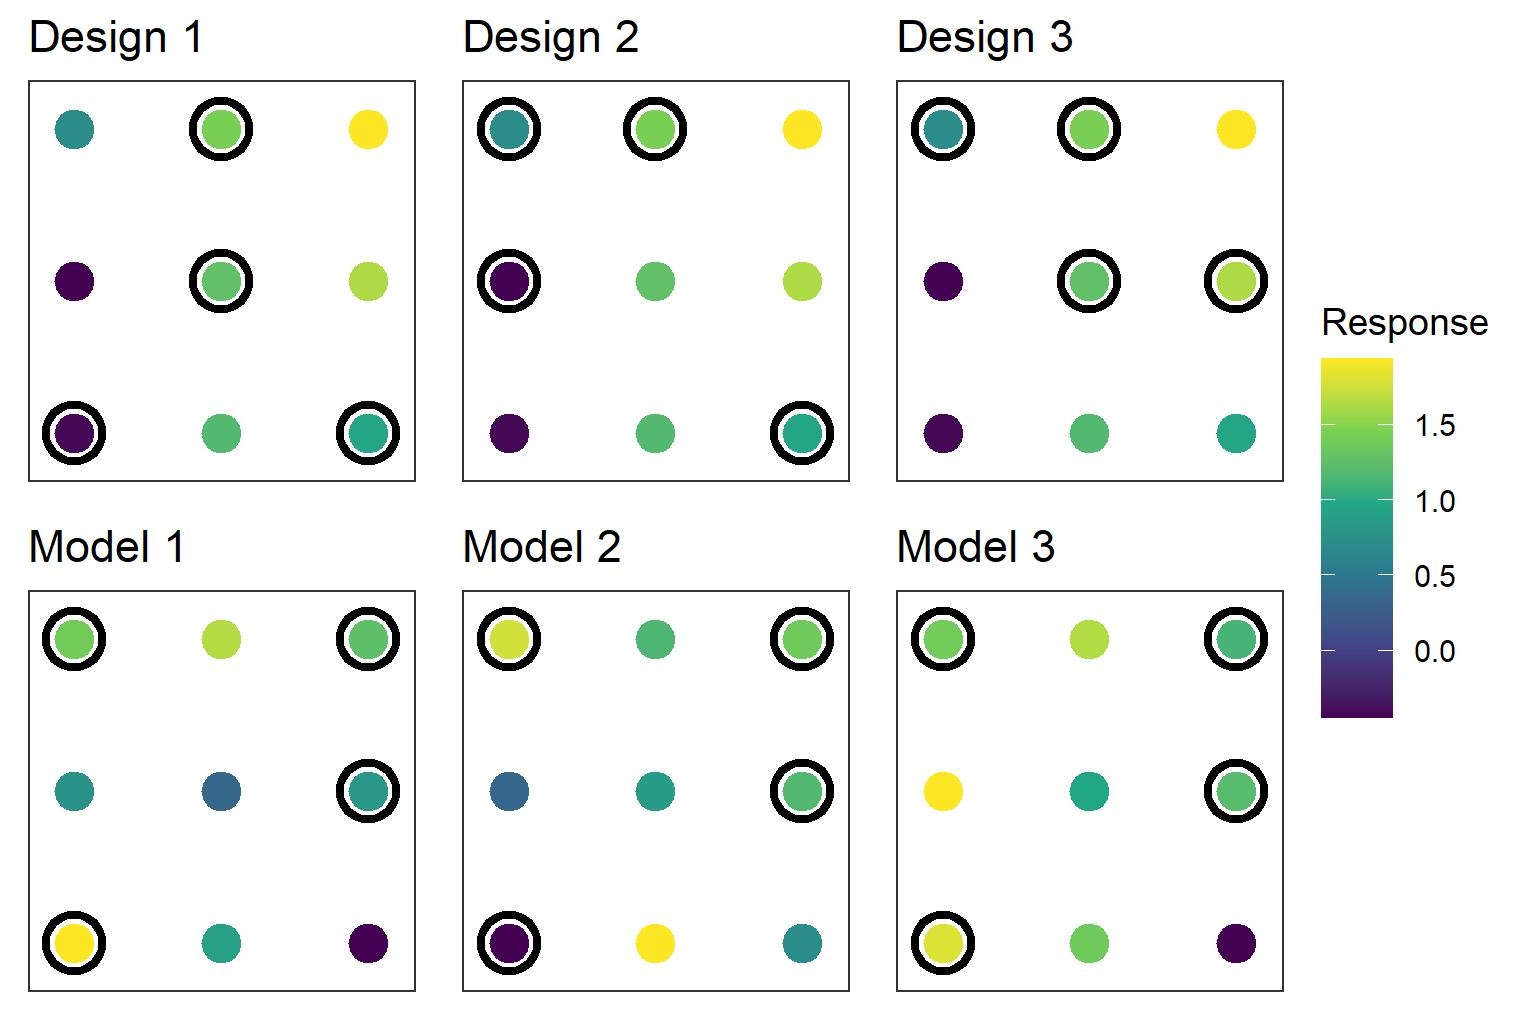
\includegraphics[width = 1\linewidth]{figures/dvm_comp.jpeg}
  \caption{A visual comparison of the design-based and model-based approaches. In the top row, the design-based approach is highlighted. There is one fixed population with nine population units and three random samples of size four (points circled are those sampled). The response values at each site are fixed. In the bottom row, the model-based approach is highlighted. There are three realizations of the same data-generating stochastic process that are all sampled at the same four locations. The response values at each site are random.}
  \label{fig:fig1}
\end{figure}

\hypertarget{subsec:spb_design}{%
\subsubsection{Spatially Balanced Design and
Analysis}\label{subsec:spb_design}}

We previously mentioned that the design-based approach can be used to
select spatially balanced samples. Spatially balanced samples are useful
because parameter estimates from these samples tend to vary less than
parameter estimates from samples lacking spatial balance (Barabesi and
Franceschi, 2011; Benedetti et al., 2017; Grafström and Lundström, 2013;
Robertson et al., 2013; Stevens and Olsen, 2004; Wang et al., 2013). The
first spatially balanced sampling algorithm to see widespread use was
the generalized random tessellation stratified (GRTS) algorithm (Stevens
and Olsen, 2004). To quantify the spatial balance of a sample, Stevens
and Olsen (2004) proposed loss metrics based on Voronoi polygons (i.e.,
Dirichlet Tessellations). After the GRTS algorithm was developed,
several other spatially balanced sampling algorithms emerged, including
stratified sampling with compact geographical strata Walvoort et al.
(2010), the local pivotal method (Grafström et al., 2012; Grafström and
Matei, 2018), spatially correlated Poisson sampling (Grafström, 2012),
balanced acceptance sampling (Robertson et al., 2013),
within-sample-distance sampling (Benedetti and Piersimoni, 2017), and
Halton iterative partitioning sampling (Robertson et al., 2018). In this
manuscript, we select spatially balanced samples using the GRTS
algorithm because it is readily available in the \texttt{spsurvey}
\textbf{\textsf{R}} package (Dumelle et al., 2022) and naturally
accommodates finite and infinite sampling frames, unequal inclusion
probabilities, and replacement units. Replacement units are additional
population units that can be sampled when a population unit originally
selected can no longer be sampled. A couple reasons why an originally
selected site can no longer be sampled include its location being
physically inaccessible or on private land that the researcher does not
have permission to access.

The GRTS algorithm selects samples by utilizing a particular mapping
between two-dimensional and one-dimensional space that preserves
proximity relationships. First the bounding box of the domain is split
up into four distinct, equally sized squares called level-one cells.
Each level-one cell is randomly assigned a level-one address of 0, 1, 2,
or 3. The set of level-one cells is denoted by \(\mathcal{A}_1\) and
defined as \(\mathcal{A}_1 \equiv \{a_1: a_1 = 0, 1, 2, 3\}\). Within
each level-one cell, the inclusion probability for each population unit
is summed, and if any of these sums exceed one, a second level of cells
is added. Then each level-one cell is split into four distinct, equally
sized squares called level-two cells. Each level-two cell is randomly
assigned a level-two address of 0, 1, 2, or 3. The set of level-two
cells is denoted by \(\mathcal{A}_2\) and defined as
\(\mathcal{A}_2 \equiv \{a_1a_2: a_1 = 0, 1, 2, 3; a_2 = 0, 1, 2, 3\}\).
The inclusion probabilities within each level-two cell are summed, and
if any of these sums exceed one, a third level of cells is added. This
process continues for \(k\) steps, until all level-\(k\) cells have
inclusion probability sums no larger than one. Then
\(\mathcal{A}_k \equiv \{a_1...a_k : a_1 = 0, 1, 2, 3; ...; a_k = 0, 1, 2, 3\}\).

After determining \(\mathcal{A}_k\), it is placed into hierarchical
order. Hierarchical order is a numeric order that first sorts
\(\mathcal{A}_k\) by the level-one addresses from smallest to largest,
then sorts \(\mathcal{A}_k\) by the level-two addresses from smallest to
largest, and so on. For example, \(\mathcal{A}_2\) in hierarchical order
is the set
\linebreak \(\{00, 01, 02, 03, 10, ..., 13, 20, ..., 23, 30, ..., 33\}\).
Because hierarchical ordering sorts by level-one cells, then level-two
cells, and so on, population units that have similar hierarchical
addresses tend to be nearby one another in space. Next each population
unit is mapped to a one-dimensional line in hierarchical order where
each population unit's inclusion probability equals its line-length. If
a level-\(k\) cell has multiple population units in it, they are
randomly placed within the cell's respective line segment. A uniform
random variable is then simulated in \([0, 1]\) and a systematic sample
is selected on the line, yielding \(n\) sample points for a sample size
\(n\). Each of these sample points falls on some population unit's line
segment, and thus that population unit is selected in the sample. For
further details regarding the GRTS algorithm, see Stevens and Olsen
(2004).

After selecting a sample and collecting data, unbiased estimates of
population means and totals can be obtained using the Horvitz-Thompson
estimator (Horvitz and Thompson, 1952). If \(\tau\) is a population
total, the Horvitz-Thompson estimator for \(\tau\), denoted by
\(\hat{\tau}_{ht}\), is is given by \begin{align}\label{eq:ht}
  \hat{\tau}_{ht} = \sum_{i = 1}^n z_i \pi_i^{-1},
\end{align} where \(z_i\) is the value of the \(i\)th population unit in
the sample, \(\pi_i\) is the inclusion probability of the \(i\)th
population unit in the sample, and \(n\) is the sample size. An estimate
of the population mean is obtained by dividing \(\hat{\tau}_{ht}\) by
\(N\), the number of population units.

It is also important to quantify the uncertainty in \(\hat{\tau}_{ht}\).
Horvitz and Thompson (1952) and Sen (1953) provide variance estimators
for \(\hat{\tau}_{ht}\), but these estimators have two drawbacks. First,
they rely on calculating \(\pi_{ij}\), the probability that population
unit \(i\) and population unit \(j\) are both in the sample -- this
quantity can be challenging if not impossible to calculate analytically
for GRTS samples. Second, these estimators tend to ignore the spatial
locations of the population units. To address these two drawbacks
simultaneously, Stevens and Olsen (2003) proposed the local neighborhood
variance estimator. The local neighborhood variance estimator does not
rely on \(\pi_{ij}\) and estimates the variance of \(\hat{\tau}\)
conditional on the random properties of the GRTS sample -- the idea
being that this conditioning should yield a more precise estimate of
\(\hat{\tau}\). They show that the contribution from each sample unit
(population unit in the sample) to the overall variance is dominated by
local variation. Thus the local neighborhood variance estimator is a
weighted sum of variance estimates from each sample unit's local
neighborhood. These local neighborhoods contain the sample unit itself
and its three nearest neighbors among all other sample units. For more
details, see Stevens and Olsen (2003).

\hypertarget{finite-population-block-kriging}{%
\subsubsection{Finite Population Block
Kriging}\label{finite-population-block-kriging}}

Finite population block kriging (FPBK) is a model-based approach that
expands the geostatistical Kriging framework to the finite population
setting (Ver Hoef, 2008). Instead of developing inference based on a
specific sampling design, we assume the data are generated by a spatial
stochastic process. We summarize some of the basic principles of FPBK
next -- for more details, see Ver Hoef (2008). Let
\({\mathbf{z} \equiv \{\text{z}(s_1), \text{z}(s_2), . . . , \text{z}(s_N) \}}\)
be an \(N \times 1\) response vector at locations \(s_1\), \(s_2\), . .
. , \(s_N\) that can be measured at the \(N\) population units. Suppose
we want to use a sample to predict some linear function of the response
variable, \(f(\mathbf{z}) = \mathbf{b}^\prime \mathbf{z}\), where
\(\mathbf{b}^\prime\) is a \(1 \times N\) vector of weights (e.g, the
population mean is represented by a weights vector whose elements all
equal \(1 / N\)). Denoting quantities that are part of the sampled
population units with a subscript \emph{s} and quantities that are part
of the unsampled population units with a subscript \emph{u}, let

\begin{equation}
\begin{pmatrix} \label{equation:Zmarginal}
    \mathbf{z}_s      \\
    \mathbf{z}_u
\end{pmatrix}
=
\begin{pmatrix}
  \mathbf{X}_s    \\
  \mathbf{X}_u
\end{pmatrix}
\bm{\beta} +
\begin{pmatrix}
\bm{\delta}_s    \\
\bm{\delta}_u
\end{pmatrix},
\end{equation} where \(\mathbf{X}_s\) and \(\mathbf{X}_u\) are the
design matrices for the sampled and unsampled population units,
respectively, \(\bm{\beta}\) is the parameter vector of fixed effects,
and \(\bm{\delta} \equiv [\bm{\delta}_s \,\, \bm{\delta}_u]'\), where
\(\bm{\delta}_s\) and \(\bm{\delta}_u\) are random errors for the
sampled and unsampled population units, respectively.

FPBK assumes \(\bm{\delta}\) in Equation\(~\)\ref{equation:Zmarginal}
has mean-zero and a spatial dependence structure that can be modeled
using a covariance function. This covariance function is commonly
assumed to be non-negative, second-order stationary (depending only on
the separation vector (e.g., distance) between population units),
isotropic (independent of direction), and decay with distance between
population units (Cressie, 1993). Henceforth, it is implied that we have
made these same assumptions regarding \(\bm{\delta}\), though Chiles and
Delfiner (1999), pp.~80-93 discuss covariance functions that are not
second-order stationary, not isotropic, or not either. A variety of
flexible covariance functions can be used to model \(\bm{\delta}\)
(Cressie, 1993); one example is the exponential covariance function
(Cressie (1993) provides a thorough list of spatial covariance
functions). The \(i,j\)th element of the exponential covariance matrix,
\(\mathop{\mathrm{{cov}}}(\bm{\delta})\), is \mbox{}
\begin{align}\label{equation:expcov}
\mathop{\mathrm{{cov}}}(\delta_i, \delta_j) = 
\begin{cases} 
\sigma^2_{1}\exp(-h_{i,j}/\phi) & h_{i,j} > 0 \\
\sigma^2_{1} + \sigma^2_2 & h_{i,j} = 0
\end{cases}
,
\end{align} where \(\sigma^2_{1}\) is the variance parameter that
quantifies the spatially dependent variability, \(\sigma^2_{2}\) is the
variance parameter the quantifies that spatially independent
variability, \(\phi\) is the distance parameter that measures the
distance-decay rate of the covariance, and \(h_{i,j}\) is the Euclidean
distance between population units \(i\) and \(j\). In geostatistical
literature, \(\sigma^2_{1}\) is often called the partial sill,
\(\sigma^2_{2}\) is often called the nugget, and \(\phi\) is often
called the range.

The parameters in Equation\(~\)\ref{equation:Zmarginal} can be estimated
using a variety of techniques, but we focus on using restricted maximum
likelihood (Harville, 1977; Patterson and Thompson, 1971; Wolfinger et
al., 1994). REML is preferred over maximum likelihood (ML) because ML
estimates can be badly biased for small sample sizes, due to the fact
that ML makes no adjustment for the simultaneous estimation of
\(\bm{\beta}\) and \(\bm{\delta}\) (Patterson and Thompson, 1971). Minus
twice the REML log-likelihood of the sampled sites is given by
\begin{equation}\label{equation:reml}
  \ln|\bm{\Sigma}| + (\bm{z}_s - \bm{X}_s \bm{\tilde{\beta}})^T \bm{\Sigma}_{ss}^{-1}(\bm{z}_s - \bm{X}_s \bm{\tilde{\beta}}) + \ln|\bm{X}_s^T \bm{\Sigma}_{ss}^{-1} \bm{X}_s| + (n - p) \ln(2 \pi) ,
\end{equation} where
\(\bm{\tilde{\beta}} = (\bm{X}_s^T \bm{\Sigma}_{ss}^{-1} \bm{X}_s)^{-1} \bm{X}_s^T \bm{\Sigma}_{ss}^{-1} \bm{z}_s\)
and \(\bm{\Sigma}_{ss}\) is the covariance matrix of the sampled sites.
Minimizing Equation\(~\)\ref{equation:reml} yields
\(\bm{\hat{\delta}}_{reml}\), the REML estimates of \(\bm{\delta}\).
Then \(\bm{\beta}_{reml}\), the REML estimate of \(\bm{\beta}\), is
given by
\((\bm{X}_s^T \bm{\hat{\Sigma}}_{ss}^{-1} \bm{X})^{-1} \bm{X}_s^T \bm{\hat{\Sigma}}_{ss}^{-1} \bm{z}_s\),
where \(\bm{\hat{\Sigma}}_{ss}\) is \(\bm{\Sigma}_{ss}\) evaluated at
\(\bm{\hat{\delta}}_{reml}\).

With the model formulation in Equation\(~\)\ref{equation:Zmarginal}, the
Best Linear Unbiased Predictor (BLUP) for \(f(\mathbf{b}'\mathbf{z})\)
and its prediction variance can be computed. While details of the
derivation are in Ver Hoef (2008), we note here that the predictor and
its variance are both moment-based, meaning that they do not rely on any
distributional assumptions. Distributional assumptions are used,
however, when constructing prediction intervals.

Other approaches, such as k-nearest-neighbors (Fix and Hodges, 1989; Ver
Hoef and Temesgen, 2013) and random forest (Breiman, 2001), among
others, could also be used to obtain predictions for a mean or total
from finite population spatial data. Compared to the k-nearest-neighbors
and random forest approach, we prefer FPBK because it is model-based and
relies on theoretically-based variance estimators leveraging the model's
spatial covariance structure, whereas k-nearest-neighbors and random
forests use ad-hoc variance estimators (Ver Hoef and Temesgen, 2013).
Additionally, Ver Hoef and Temesgen (2013) compared FPBK,
k-nearest-neighbors, and random forest in a variety of spatial data
contexts, and FPBK tended to perform best.

\hypertarget{sec:mm}{%
\section{Materials and Methods}\label{sec:mm}}

In this section we describe how we used simulated and real data to
investigate performance between simple random sampling without
replacement (SRS) and GRTS sampling as well as performance between
design-based (DB) and model-based (MB) inference. In SRS and GRTS
sampling, all population units had equal inclusion probabilities. The
important distinction between SRS and GRTS is that SRS ignores spatial
locations while sampling but GRTS explicitly incorporates them.
Together, the two sampling plans (SRS and GRTS) combined with the two
inference approaches (DB and MB) yielded four sampling-inference
combinations: SRS-DB, SRS-MB, GRTS-DB, and GRTS-MB. For SRS-DB, the
Horvitz-Thompson estimator \eqref{eq:ht} was used to estimate means and
the commonly-used SRS variance formula (Lohr, 2009; Särndal et al.,
2003) was used to estimate the variance. This variance formula is given
by \begin{equation}\label{equation:srs_var}
 \frac{f[\sum_{i = 1}^n (z_i - \bar{z})^2]}{n(n - 1)},
\end{equation} where \(z_i\) is the \(i\)th response value, \(\bar{z}\)
is the mean of all \(z_i\), \(n\) is the sample size, \(N\) is the
population size, and \(f = (1 - n / N)\) (\(f\) is often called the
finite population correction factor). For GRTS-DB, the Horvitz-Thompson
esetimator was used to estimate means and the local neighborhood
variance was used to estimate variances. For SRS-MB and GRTS-MB, FPBK
was used to estimate means and variances and parameters were estimated
using restricted maximum likelihood.

We used simulated data to compare the sampling-inference combinations
across many realized populations from the same data-generating
stochastic process. With the simulated data, we were in control of the
data-generating stochastic process and the random sampling process. We
used real data from the 2012 National Lakes Assessment (USEPA, 2012) to
compare the sampling-inference combinations within a single realized
population (which is typically the case in reality). With the real data,
we were in control of only the random sampling process.

\hypertarget{sec:mm_sim}{%
\subsection{Simulated Data}\label{sec:mm_sim}}

We evaluated performance of the four sampling-inference combinations in
36 different simulation scenarios. The 36 scenarios resulted from the
crossing of three sample sizes, two location layouts (of the population
units), two response types, and three proportions of dependent random
error (DRE). The three sample sizes (\(n\)) were \(n = 50, n = 100,\)
and \(n = 200\). Samples were always selected from a population size
(\(N\)) of \(N = 900\). The two location layouts were random and
gridded. Locations in the random layout were randomly generated inside
the unit square (\([0, 1] \times [0, 1]\)). Locations in the gridded
layout were placed on a fixed, equally spaced grid inside the unit
square. The two response types were normal and skewed. For the normal
response type, the response was simulated using mean-zero random errors
with the exponential covariance (Equation\(~\)\ref{equation:expcov}) for
three proportions of dependent random error (DRE): 0\% DRE, 50\% DRE,
and 90\% DRE. Recall the proportion of DRE is represented by
\(\sigma^2_1 / (\sigma^2_1 + \sigma^2_2)\), where \(\sigma^2_1\) and
\(\sigma^2_2\) are the DRE variance and independent random error (IRE)
variance from Equation\(~\)\ref{equation:expcov}, respectively. The
total variance, \(\sigma^2_1 + \sigma^2_2\), was always 2. The distance
parameter was always \(\sqrt{2} / 3\), chosen so that the correlation in
the DRE decayed to nearly zero at \(\sqrt{2}\), the largest possible
distance between two population units in the domain. For the skewed
response type, the response was first simulated using the same approach
as for the normal response type, except that the total variance was
0.6931 instead of 2. The response was then exponentiated, yielding a
skewed random variable whose total variance was 2. The skewed responses
were used to evaluate performance of the sampling-inference approaches
for data that were not normal but were still estimated using REML, which
relies on a normal log-likelihood. Figure \ref{fig:sim_pops} shows an
example of a realized population for the normal and skewed responses
using the random layout and 50\% DRE.

\begin{figure}
\centering
\begin{subfigure}{0.49\textwidth}
  \centering
  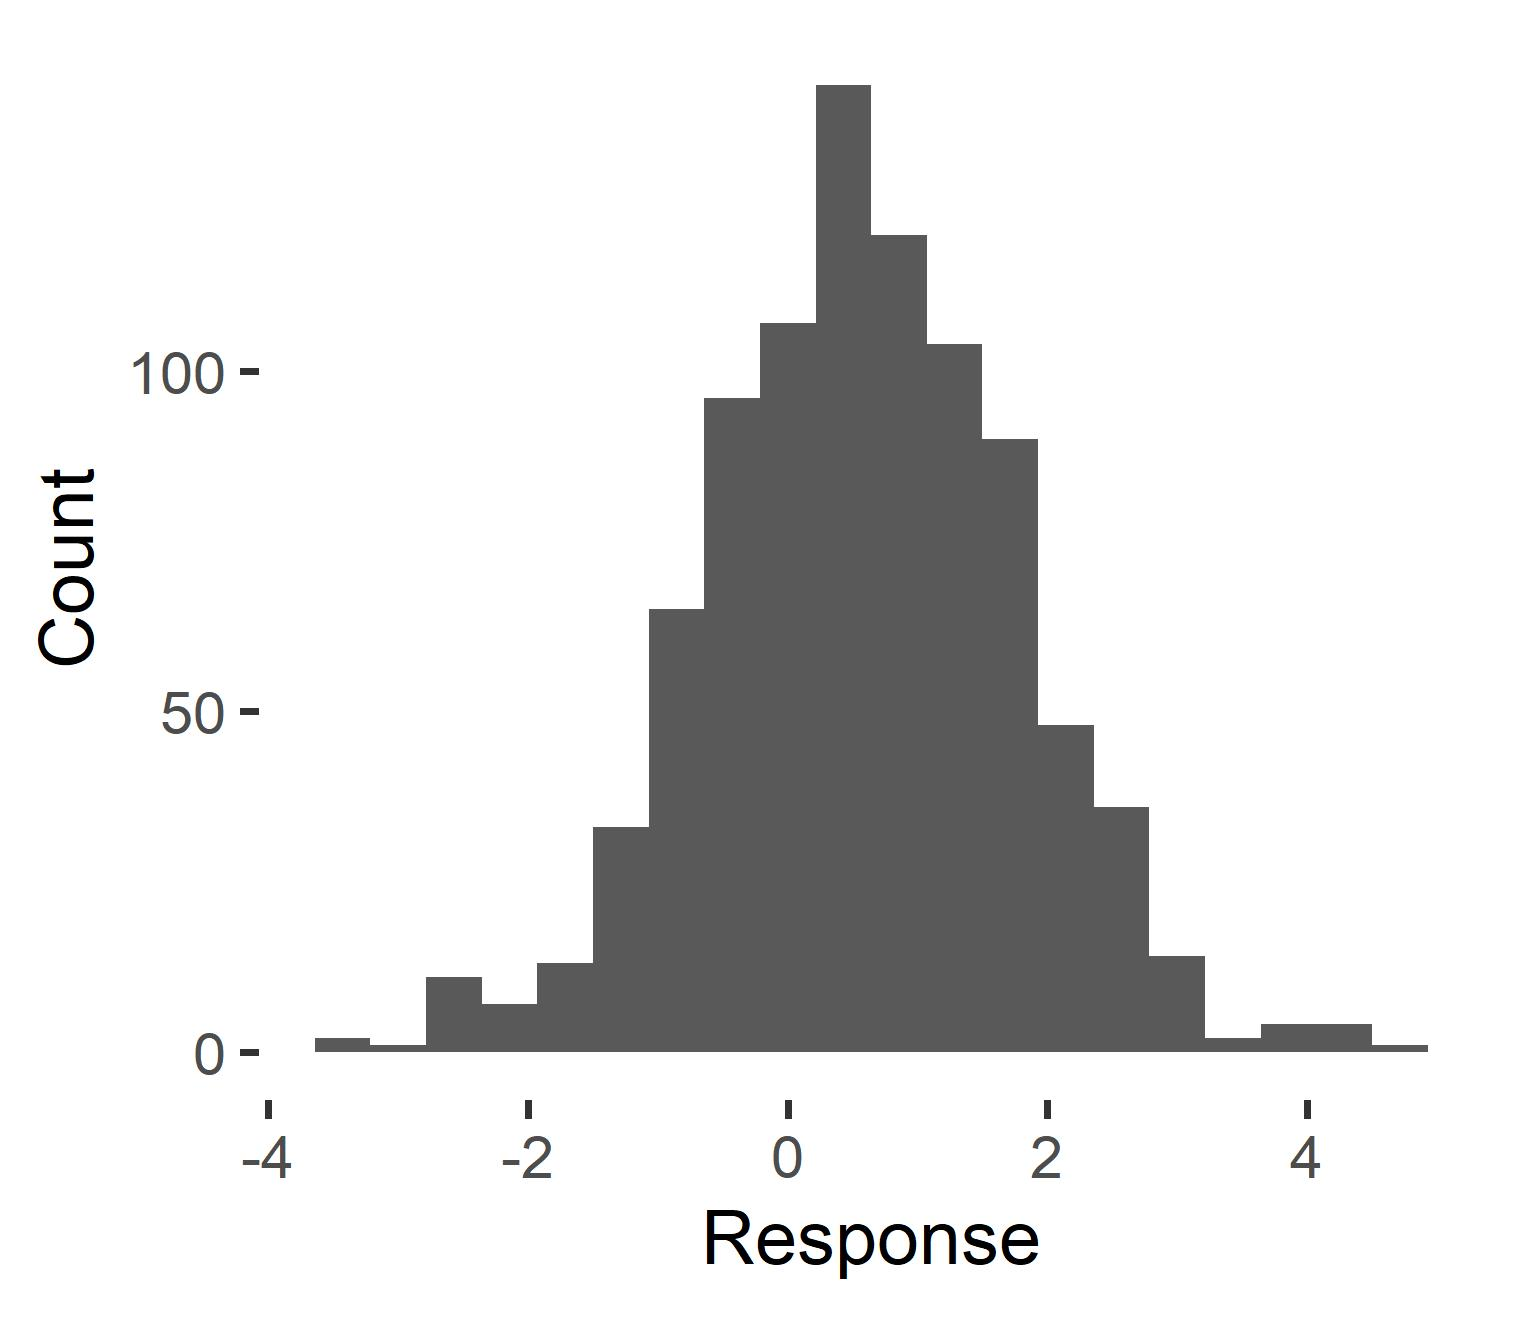
\includegraphics[width = 1\linewidth]{figures/symm_pop_hist.jpeg}
  \caption{Histogram of a realized population for the normal response.}
  \label{fig:symm_pop_hist}
\end{subfigure}
\begin{subfigure}{0.49\textwidth}
  \centering
  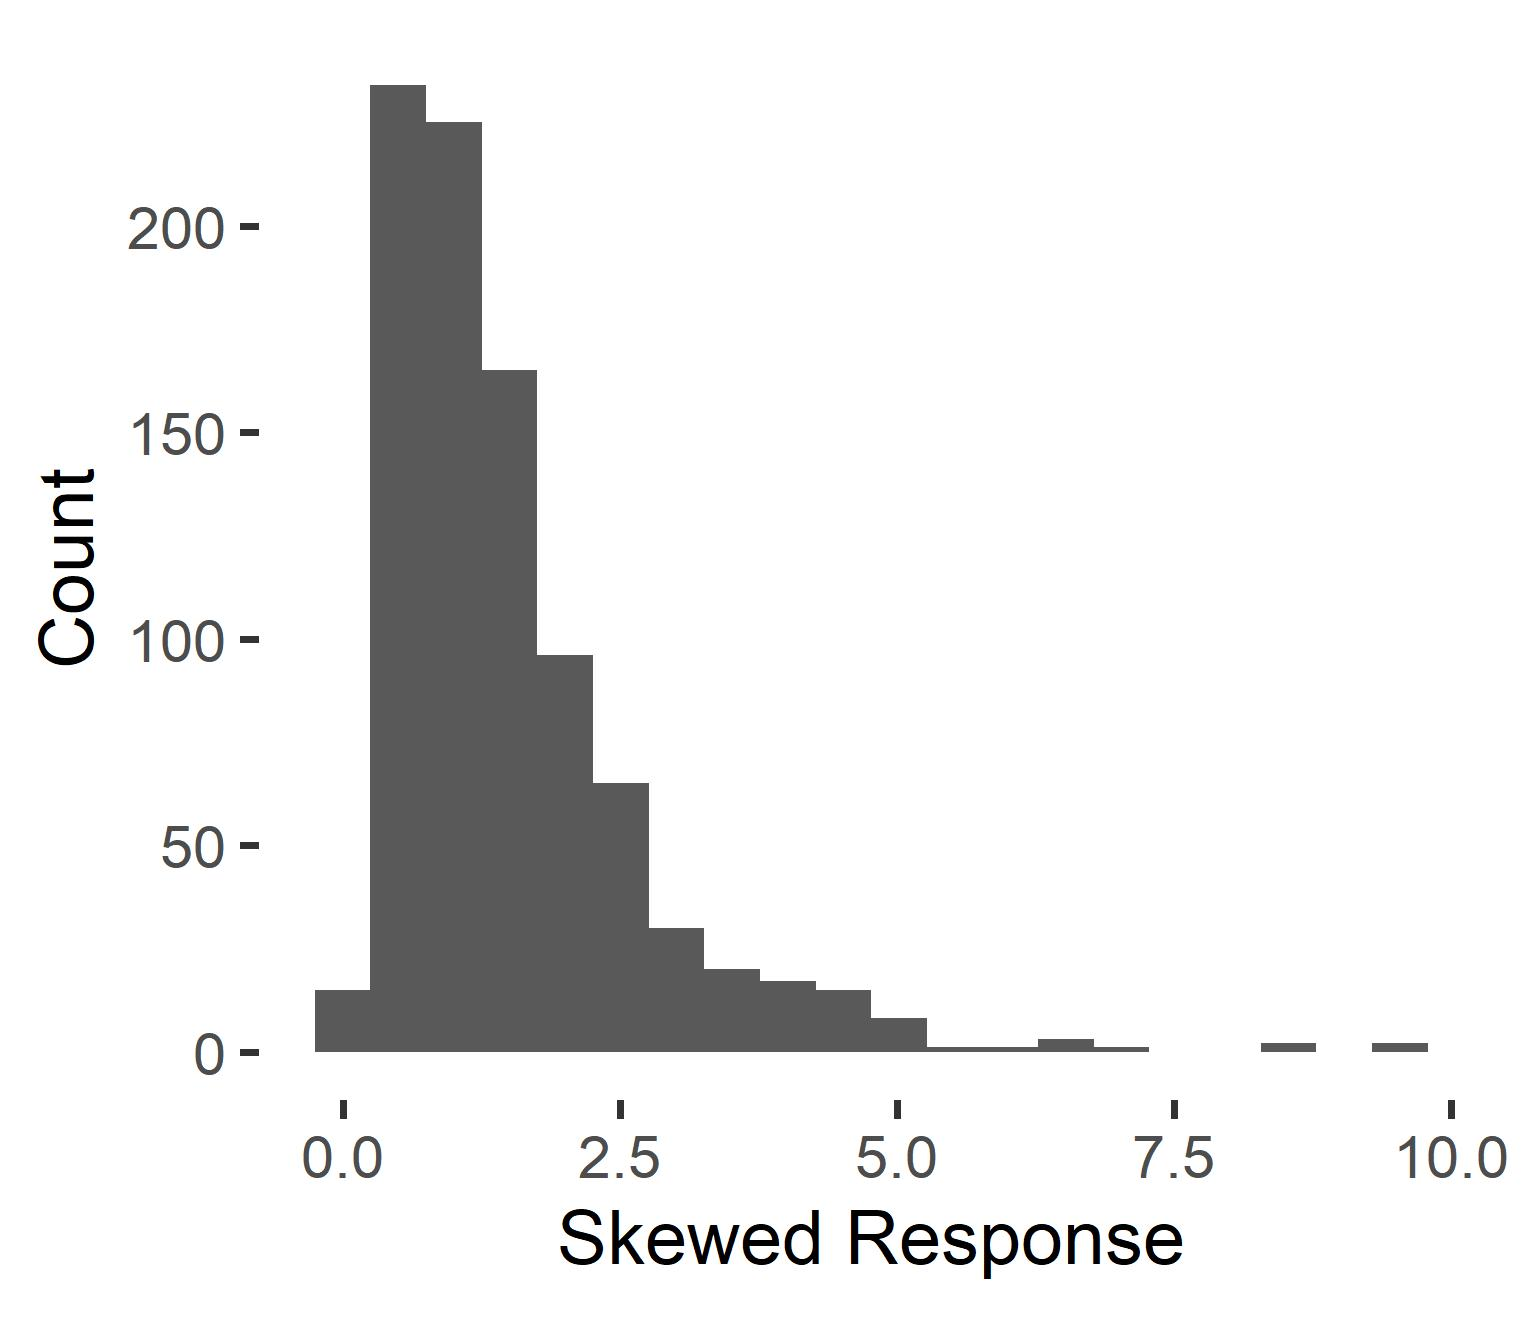
\includegraphics[width = 1\linewidth]{figures/skew_pop_hist.jpeg}
  \caption{Histogram of a realized population for the skewed response.}
  \label{fig:skew_pop_hist}
\end{subfigure}
\caption{Histograms of realized populations simulated for the normal and skewed resposnes using the random layout and 50\% DRE.}
\label{fig:sim_pops}
\end{figure}

In each of the 36 simulation scenarios, there were 2000 independent
simulation trials. Within each simulation scenario and trial, IRS and
GRTS samples were selected and then design-based and model-based
analyses were used to estimate (design-based) or predict (model-based)
the mean and construct 95\% confidence (design-based) or 95\% prediction
(model-based) intervals. With the model-based analyses, covariance
parameters were estimated (using REML) separately for each trial. After
all 2000 trials, we summarized the long-run performance of the
sampling-inference combination in each scenario by calculating mean
bias, root-mean-squared error, and interval coverage. Mean bias is taken
as the average deviation between each trial's estimated (or predicted)
mean and its realized mean:
\(\frac{1}{n}\sum_{i = 1}^{2000} (\hat{\mu}_i - \mu_i)\), where \(i\)
indexes simulation trials. Root-mean-squared error is taken as the
square root of the average squared deviation between each trial's
estimated (or predicted) mean and its realized mean:
\(\sqrt{\frac{1}{n}\sum_{i = 1}^{2000} (\hat{\mu}_i - \mu_i)^2}\).
Interval coverage is taken as the proportion of simulation trials where
the realized mean is contained in its 95\% confidence (or prediction)
interval. These intervals are constructed using the normal distribution
-- justification comes from the asymptotic normality of means via the
central limit theorem (under some assumptions). Quantifying these
metrics is important because together, they give us an idea of the
accuracy (mean bias), spread (RMSE), and validity (interval coverage) of
the sampling-inference combinations.

\hypertarget{sec:mm_app}{%
\subsection{National Lakes Assessment (Real) Data}\label{sec:mm_app}}

The United States Environmental Protection Agency (USEPA), states, and
tribes periodically conduct National Aquatic Research Surveys (NARS) to
assess the water quality of various bodies of water in the contiguous
United States. One component of NARS is the National Lakes Assessment
(NLA), which measures various aspects of lake health and water quality.
We focus on analyzing zooplankton multi-metric indices (ZMMI) and
mercury concentrations in parts per billion (Hg ppb) from the 2012 NLA.
For ZMMI, data were collected at 1035 unique lakes. At less than 10\% of
lakes, two ZMMI replicates were collected. These were averaged for the
purposes of our study so that each lake had one measurement for ZMMI.
For Hg ppb, data were collected at 995 unique lakes (and there were no
replicates like for ZMMI). The ZMMI and Hg ppb data are shown as spatial
maps and as histograms in Figure \ref{fig:zmmi}. The ZMMI data tend to
be highest near the coasts, lowest in the Central United States, higher
near the coasts, are relatively symmetric, and have a mean of 55.05. The
Hg ppb data tend to be highest in the Northeastern United States, lowest
elsewhere, are skewed, and have a mean of 103.16 ppb. Also in Figure
\ref{fig:zmmi} are separate spatial semivariograms for ZMMI and Hg ppb.
The spatial semivariogram quantifies the the halved average squared
differences (semivariance) of responses whose separation (distance)
falls within some distance class. The spatial semivariance is closely
related to the spatial covariance, and spatial semivariograms are often
used to gauge the strength of spatial dependence in data. Both ZMMI and
Hg ppb seem to have moderately strong spatial dependence (Figure
\ref{fig:zmmi}), as the semivariance increases steadily with distance
(meaning that observations nearby one another tend to be more similar
than observations far apart from one another).

\begin{figure}
\centering
\begin{subfigure}{0.49\textwidth}
  \centering
  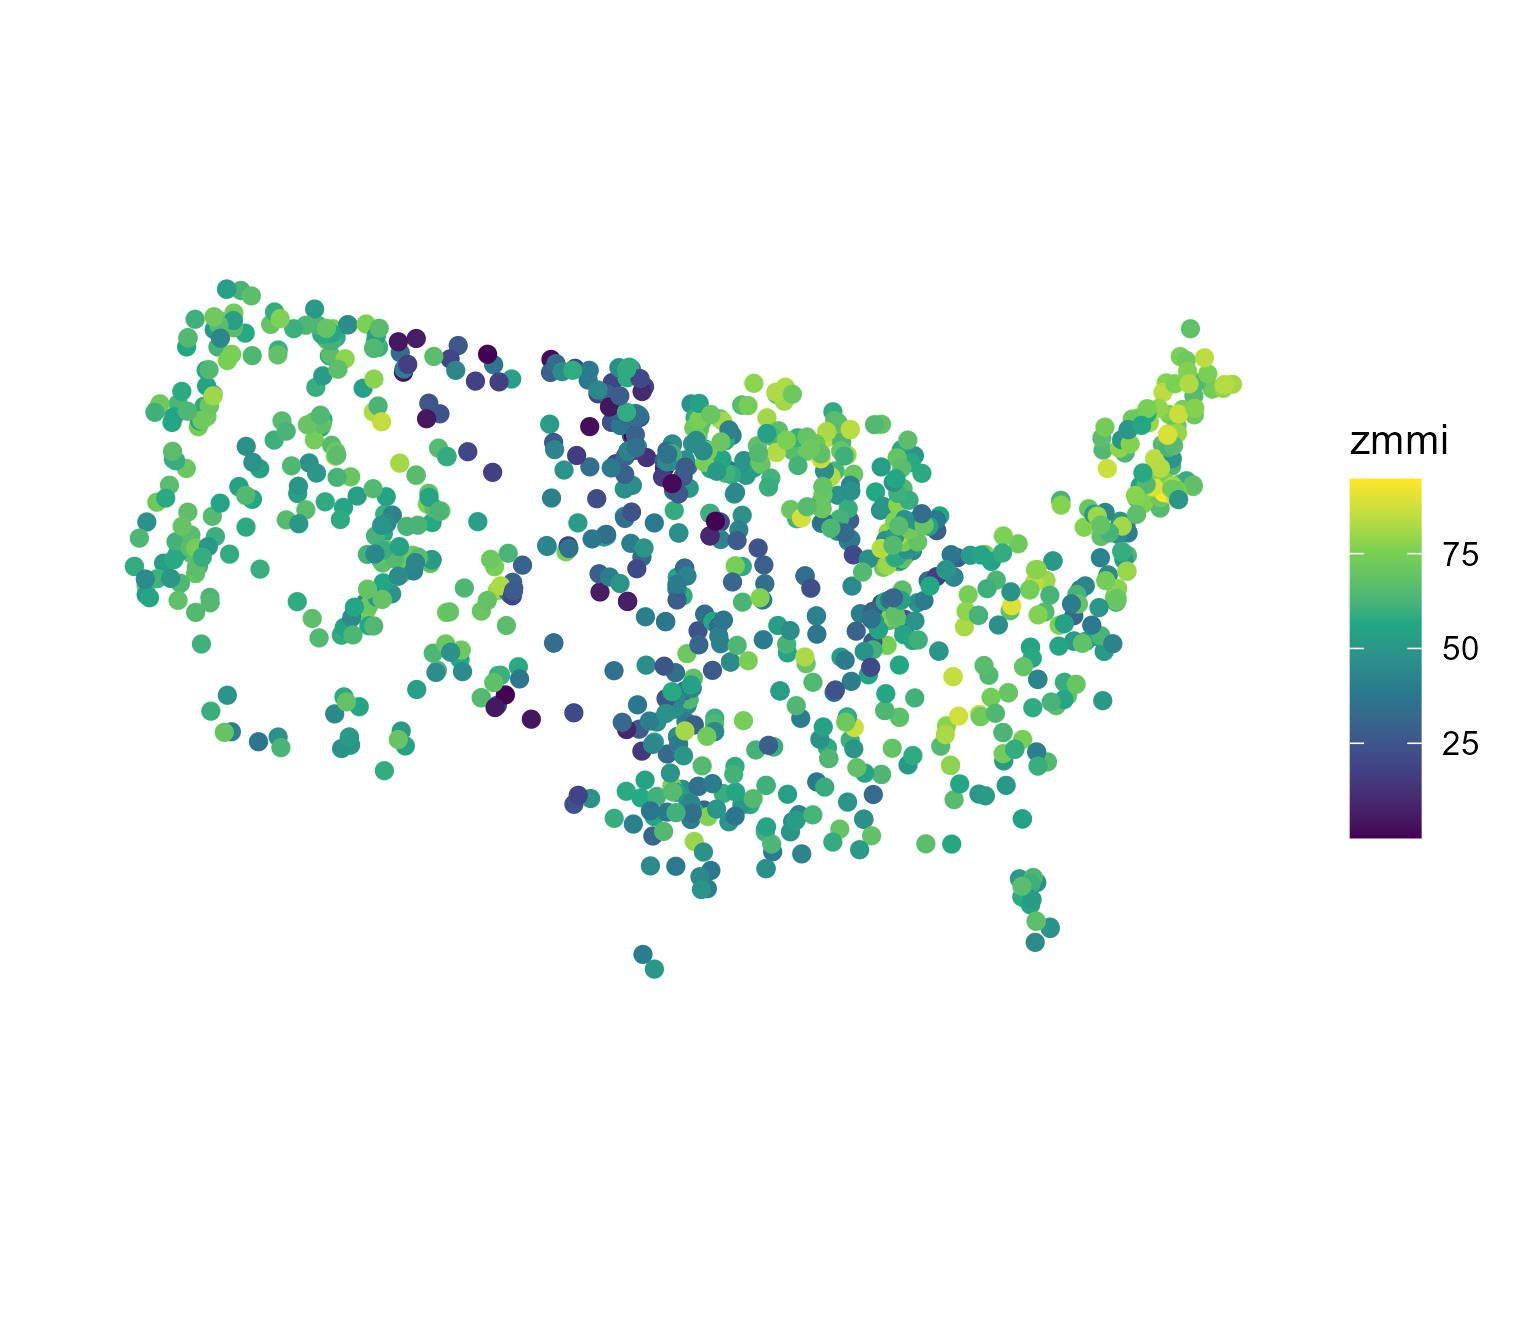
\includegraphics[width = 1\linewidth]{figures/zmmi_map.jpeg}
  \caption{Spatial map of the ZMMI population.}
  \label{fig:zmmi_map}
\end{subfigure}
\begin{subfigure}{0.49\textwidth}
  \centering
  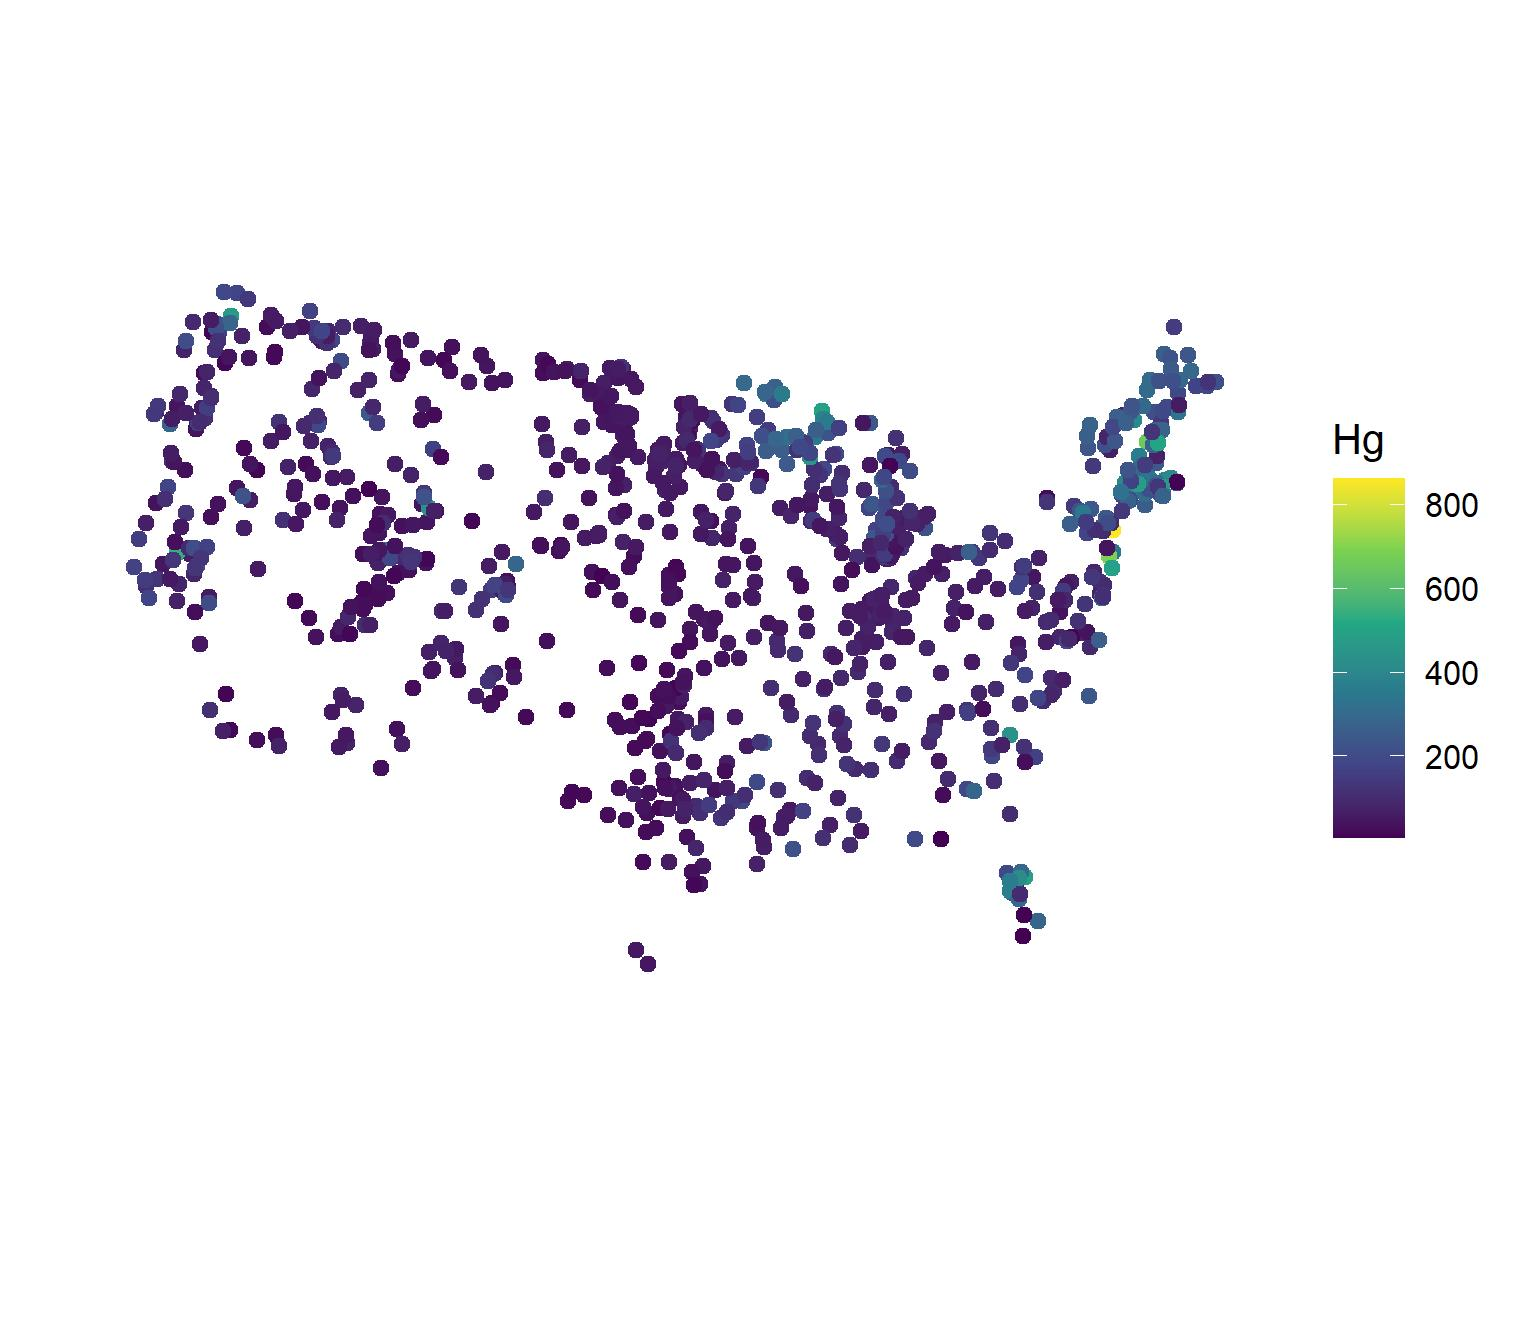
\includegraphics[width = 1\linewidth]{figures/mercury_map.jpeg}
  \caption{Spatial map of mercury (Hg ppb) population.}
  \label{fig:mercury_map}
\end{subfigure} \\
\begin{subfigure}{0.49\textwidth}
  \centering
  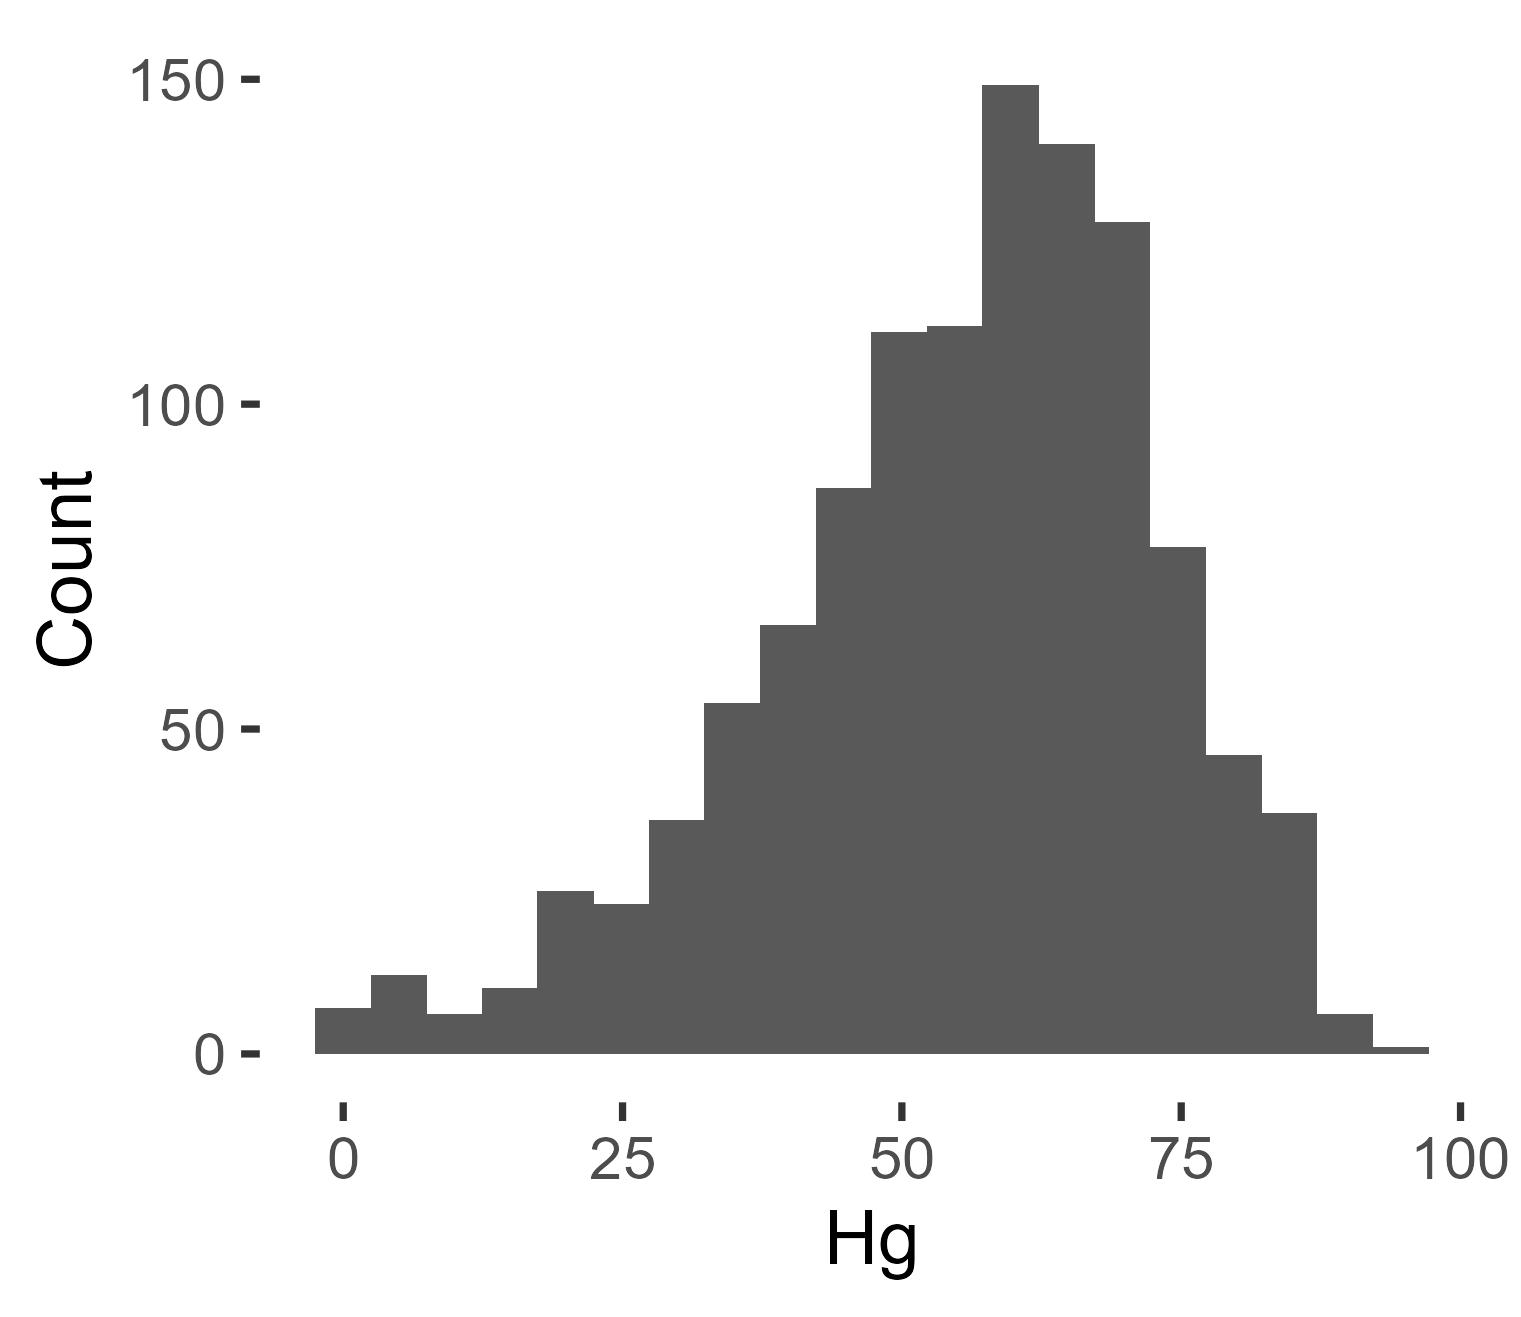
\includegraphics[width = 1\linewidth]{figures/zmmi_hist.jpeg}
  \caption{Histogram of the ZMMI population.}
  \label{fig:zmmi_hist}
\end{subfigure}
\begin{subfigure}{0.49\textwidth}
  \centering
  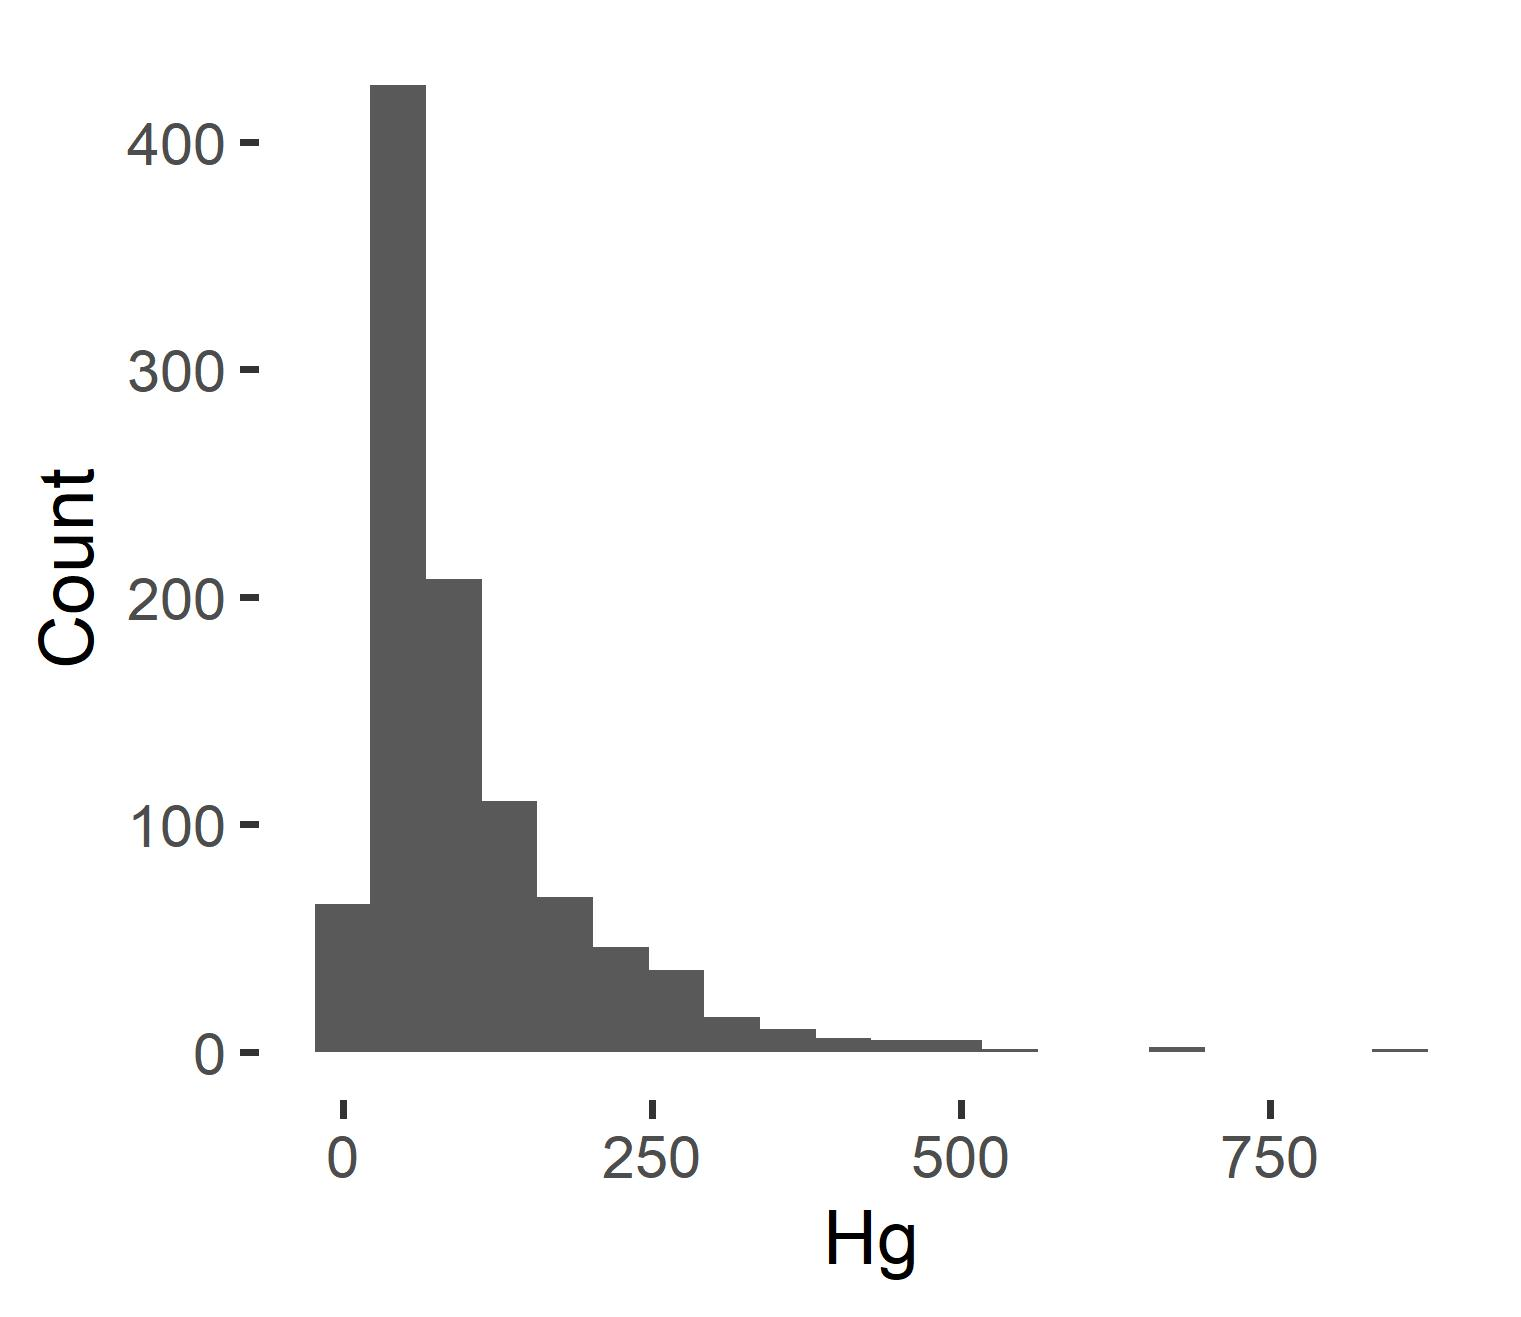
\includegraphics[width = 1\linewidth]{figures/mercury_hist.jpeg}
  \caption{Histogram of the mercury (Hg ppb) population.}
  \label{fig:mercury_hist}
\end{subfigure} \\
\begin{subfigure}{0.49\textwidth}
  \centering
  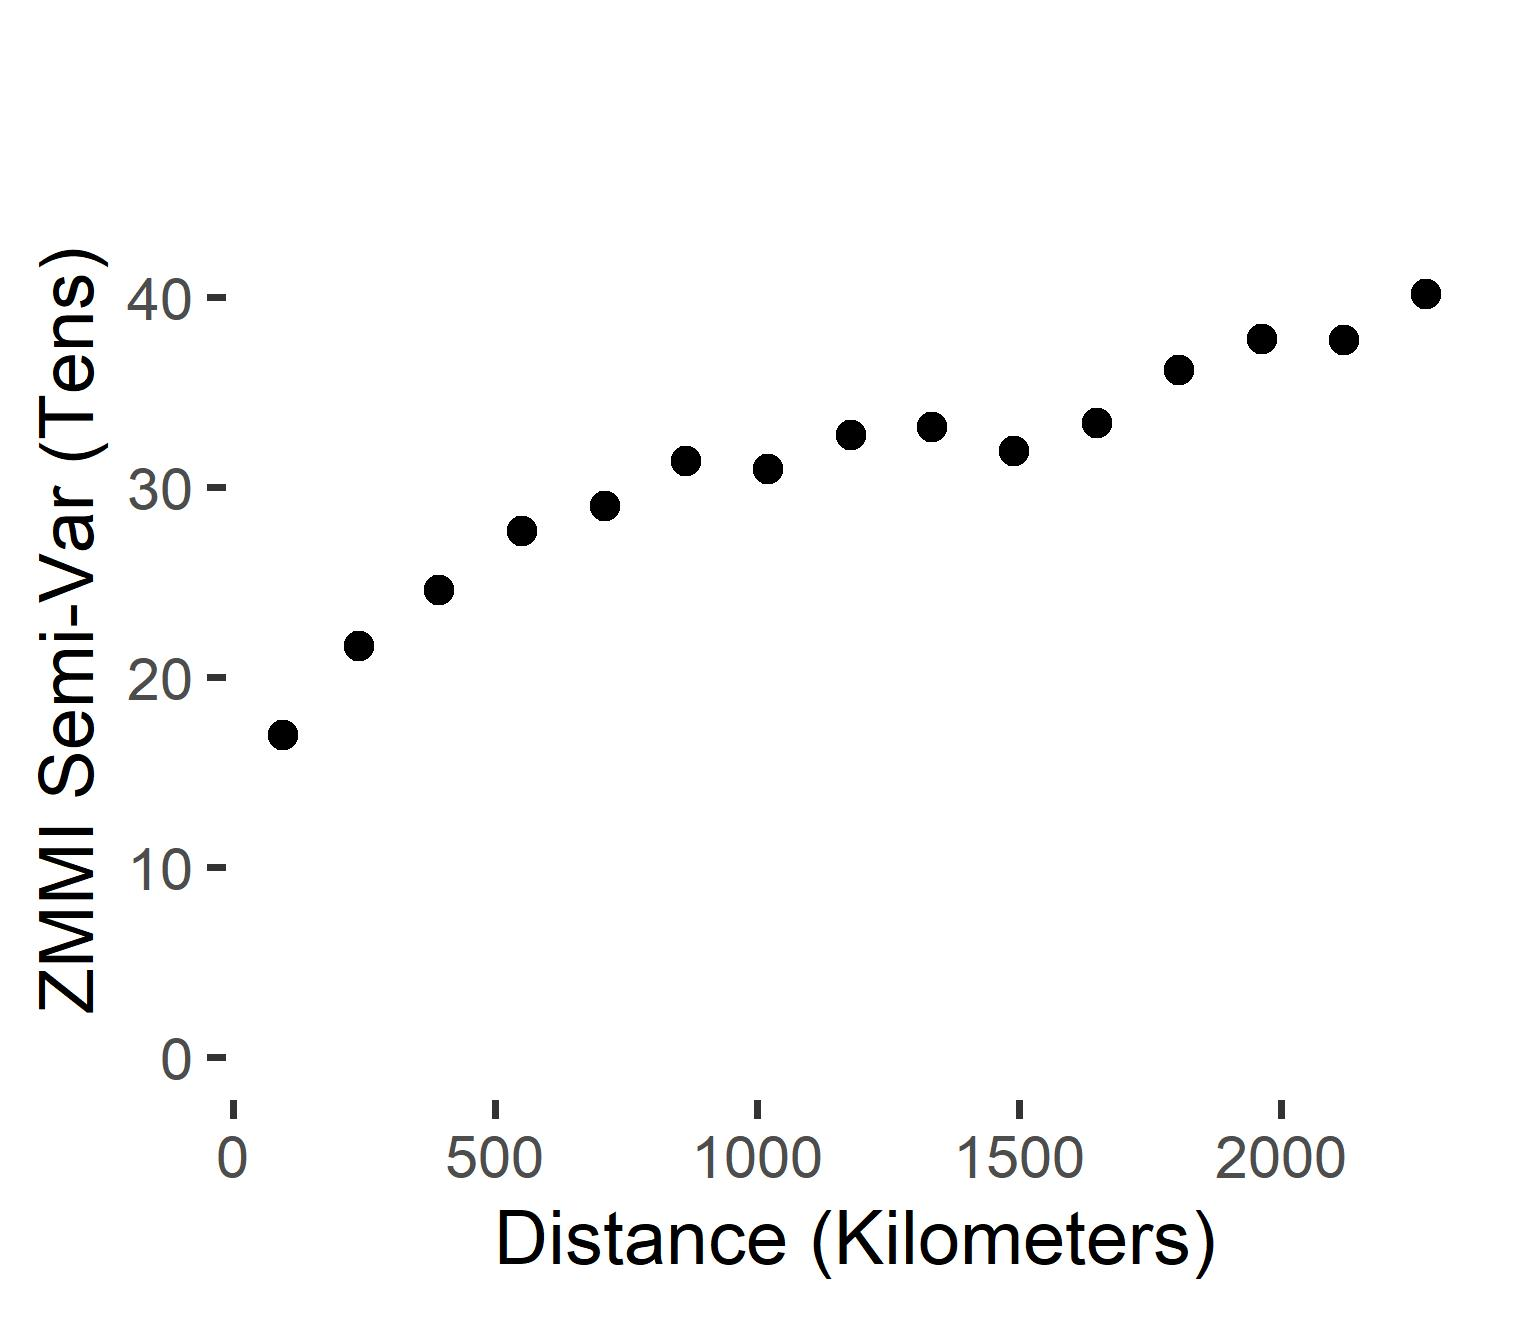
\includegraphics[width = 1\linewidth]{figures/zmmi_sv.jpeg}
  \caption{Semivariogram of the ZMMI population.}
  \label{fig:zmmi_sv_plot}
\end{subfigure}
\begin{subfigure}{0.49\textwidth}
  \centering
  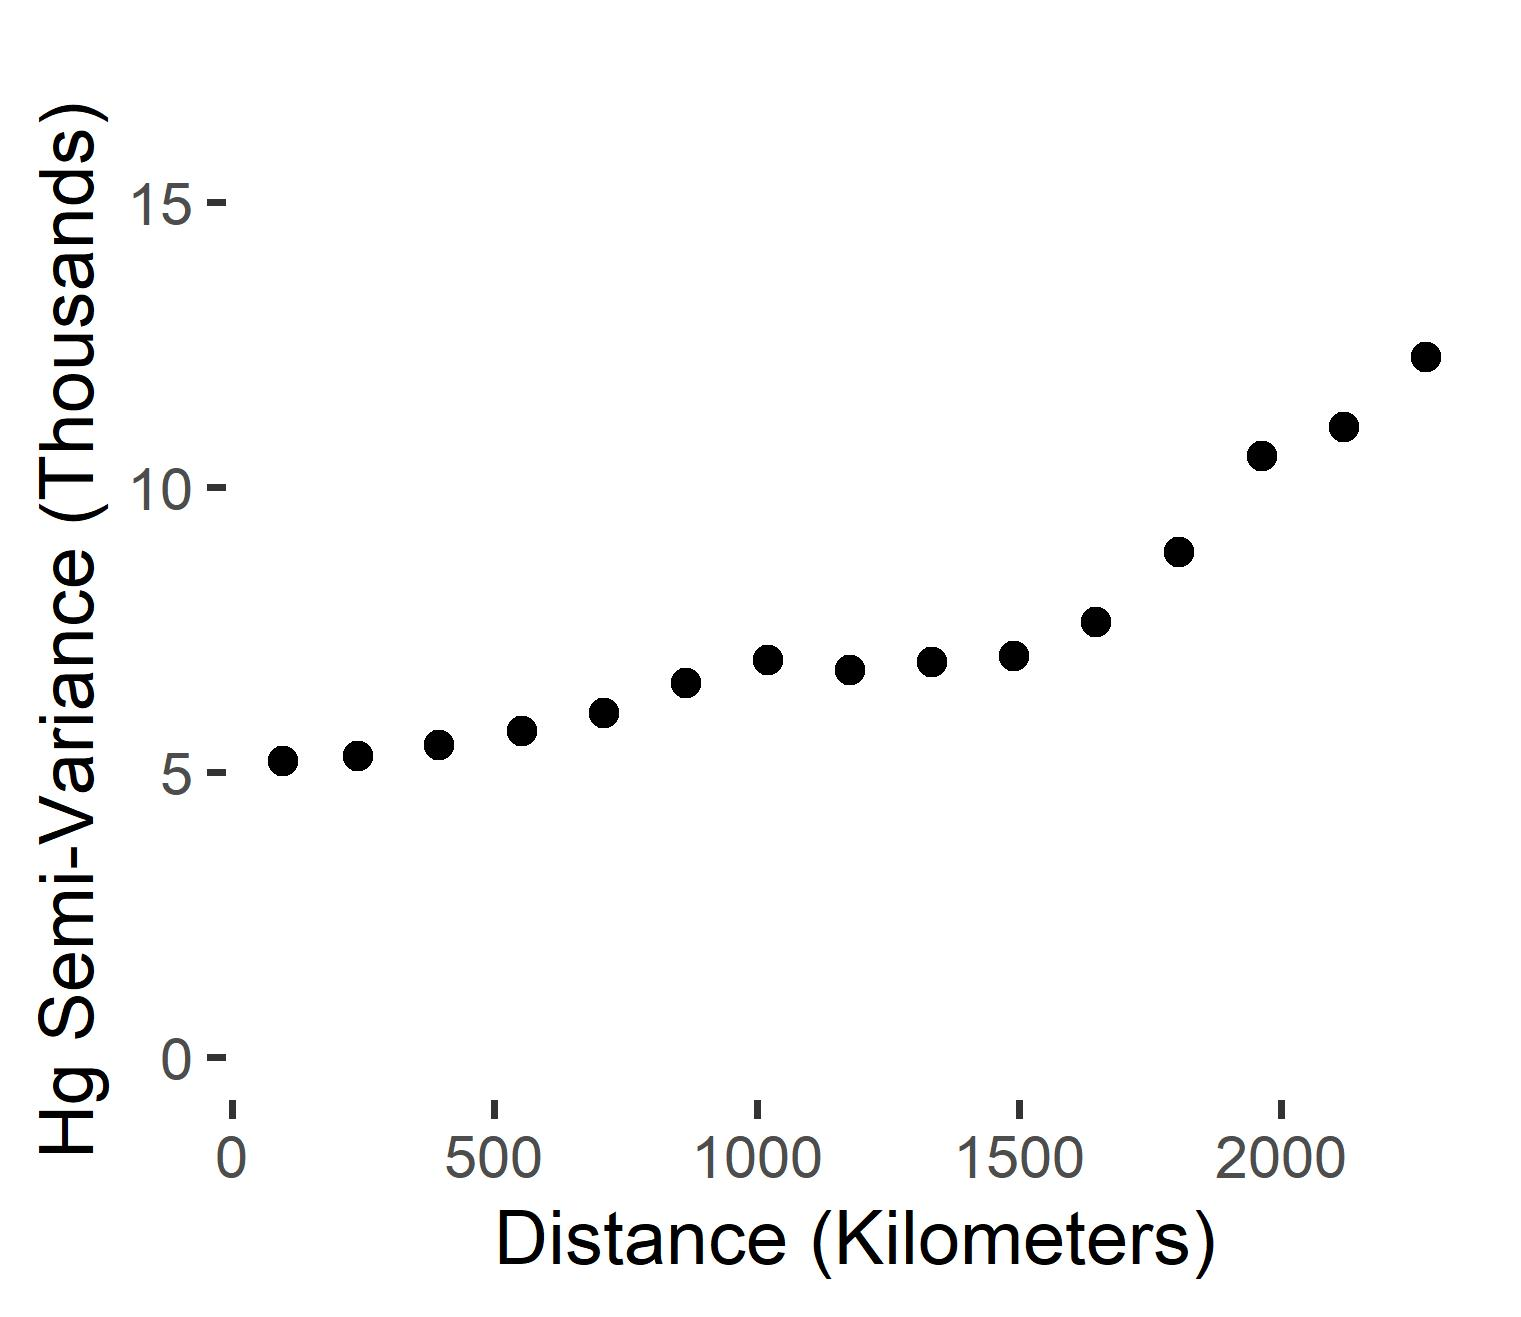
\includegraphics[width = 1\linewidth]{figures/mercury_sv.jpeg}
  \caption{Semivariogram of the mercury (Hg ppb) population.}
  \label{fig:mercury_sv_plot}
\end{subfigure}
\caption{Exploratory graphics of the ZMMI and mercury (Hg ppb) populations in the National Lakes Assessment (NLA) 2012 data.}
\label{fig:zmmi}
\end{figure}

We studied performance of the four sampling-inference combinations by
selecting 2000 random IRS and GRTS samples of size \(n = 50\),
\(n = 100\), and \(n = 200\) from the realized ZMMI and Hg ppb
populations and then analyzing the samples using MB and DB inference. In
total, there were six separate scenarios (two responses and three sample
sizes). We used the same evaluation metrics as for the simulated data:
mean bias, RMSE, and interval coverage. Mean bias is taken as the
average deviation between each sample's estimated (or predicted) mean
and the population mean (of ZMMI or Hg ppb):
\(\frac{1}{n}\sum_{i = 1}^{2000} (\hat{\mu}_i - \mu)\), where \(i\)
indexes simulation trials and \(\mu\) is the population mean.
Root-mean-squared error is taken as the square root of the average
squared deviation between each sample's estimated (or predicted) mean
and its population mean:
\(\sqrt{\frac{1}{n}\sum_{i = 1}^{2000} (\hat{\mu}_i - \mu)^2}\).
Interval coverage is taken as the proportion of simulation trials where
the population mean is contained in its 95\% confidence (or prediction)
interval. These intervals are constructed using the normal distribution.

\hypertarget{sec:results}{%
\section{Results}\label{sec:results}}

\hypertarget{sec:r_sim}{%
\subsection{Simulated Data}\label{sec:r_sim}}

Mean bias was nearly zero for all four sampling-inference combinations
in all 36 scenarios, so we omit a more detailed summary of those results
here. Tables for mean bias in all 36 simulation scenarios are provided
in the supporting information.

We define the relative RMSE as a ratio with numerator given by the RMSE
for a sampling-inference combination and the denominator given by the
RMSE for SRS-DB. Relative RMSEs for the random location layout are
provided in Fig. \ref{fig:rmspe_eff}. When there is no spatial
covariance (Fig. \ref{fig:rmspe_eff}, ``DRE\%: 0\%''), the four
sampling-inference combinations have approximately equal RMSE. In these
scenarios, using GRTS sampling or model-based inference does not
generally increase efficiency compared to SRS-DB. When there is spatial
covariance (Fig. \ref{fig:rmspe_eff}, ``DRE\%: 0\%'' and ``DRE\%:
50\%''), GRTS-MB tends to have the lowest RMSE, followed by GRTS-DB,
SRS-MB, and finally SRS-DB, though the difference in relative RMSE among
GRTS-MB, GRTS-DB, and SRS-MB is small. As the strength of spatial
covariance increases, the gap in RMSE between SRS-DB and the other
sampling-inference combinations widens. Finally we note that when there
is spatial covariance, SRS-MB has a much lower RMSE than SRS-DB,
suggesting that the lack of efficiency from SRS is largely mitigated by
model-based inference. These RMSE conclusions are similar to those
observed in the grid location layout, so we omit a figure and discussion
regarding the grid location layout here. Tables for RMSE in all 36
simulation scenarios are provided in the supporting information.

\begin{figure}
  \centering
  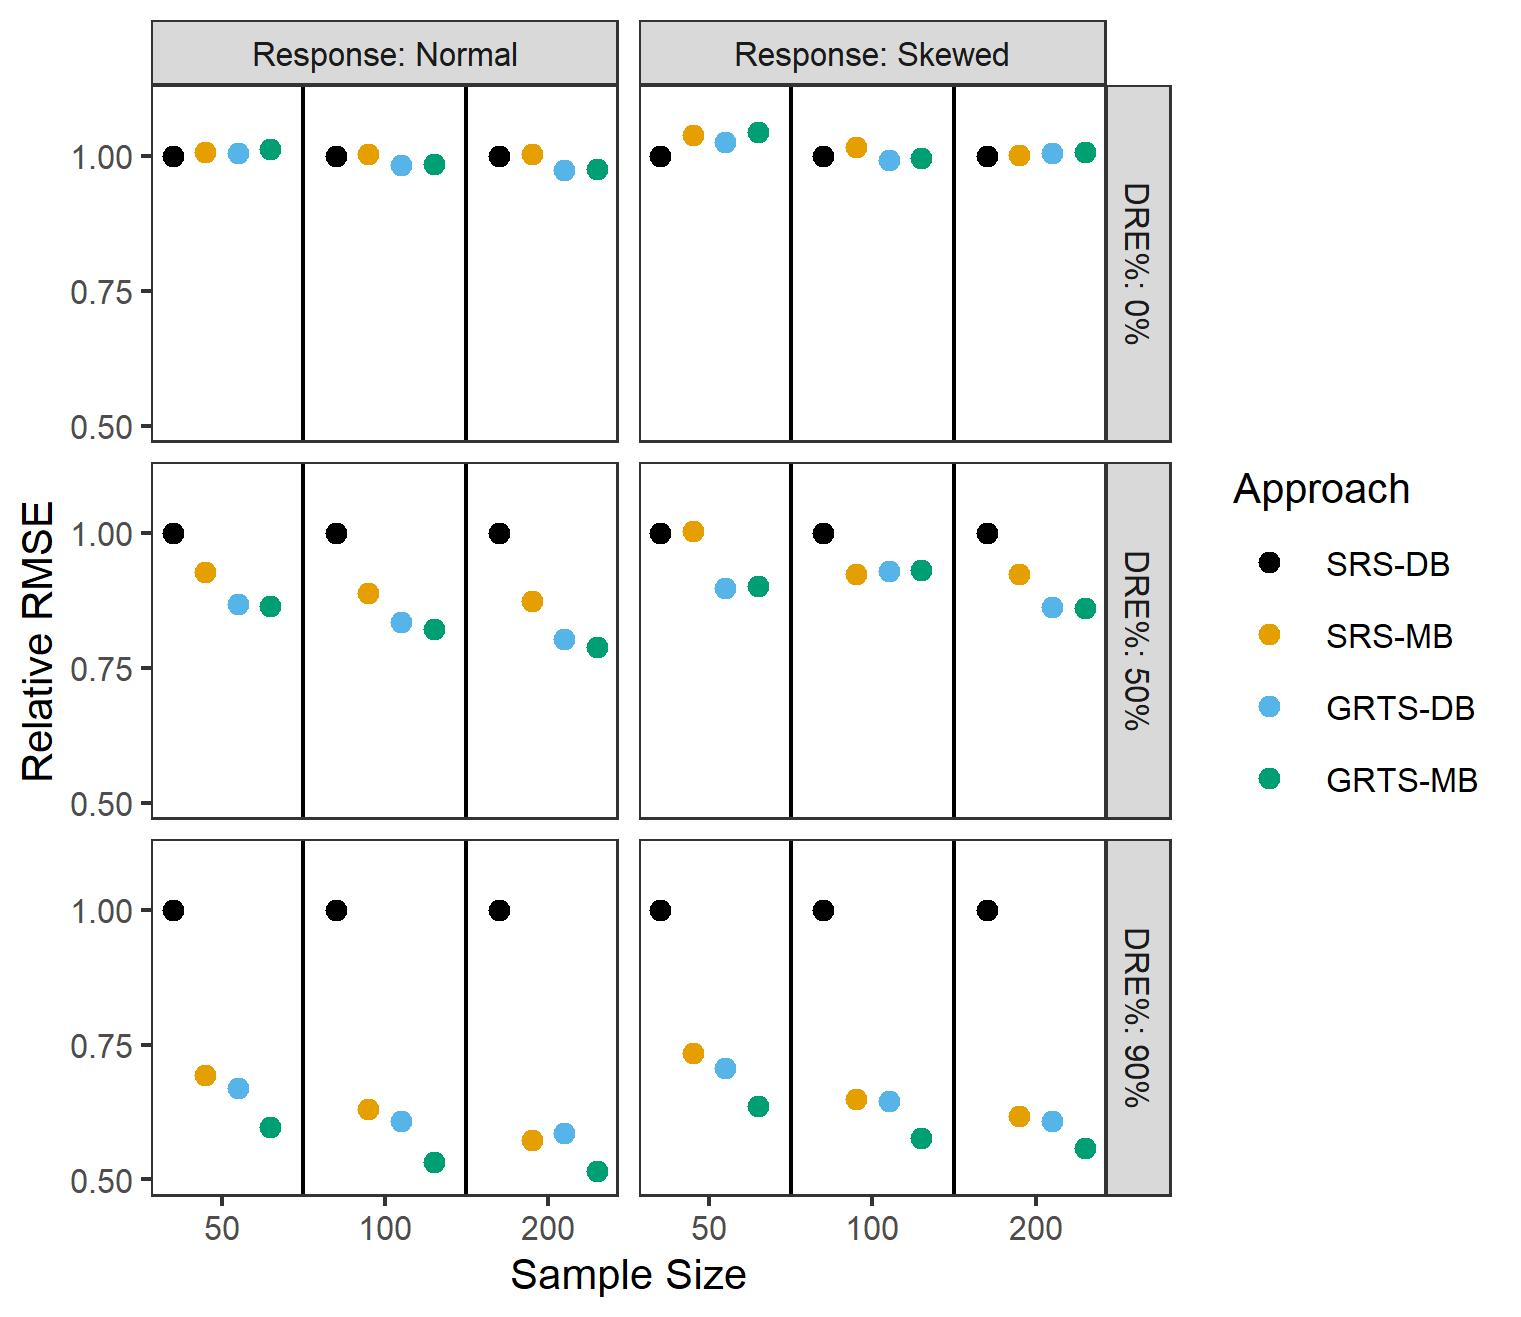
\includegraphics[width = 1\linewidth]{figures/rmspe_eff.jpeg}
  \caption{Relative RMSE in the simulation study for the four sampling-inference combinations and three sample sizes in the random location layout. The rows indicate the proportion of dependent error and the columns indicate the response type. The solid, black lines separate the sample sizes.}
  \label{fig:rmspe_eff}
\end{figure}

95\% interval coverage for each of the four sampling-inference
combinations in the random location layout is shown in Fig.
\ref{fig:figconf}. Within each simulation scenario, all
sampling-inference combinations tend to have fairly similar interval
coverage, though when \(n = 50\) or \(n = 100\), GRTS-DB coverage is
usually a few percentage points lower than the other combinations, which
suggests that the local neighborhood variance estimate may be slightly
too small for small \(n\). Coverage in the normal response scenarios was
usually near 95\%, while coverage in the skewed response scenarios
usually varied from 90\% to 95\% but increased with the sample size. At
a sample size of 200, all four sampling-inference combinations had
approximately 95\% interval coverage in both response scenarios for all
dependent error proportions. These interval coverage conclusions are
similar to those observed in the grid location layout, so we omit a
figure and discussion regarding the grid location layout here. Tables
for interval coverage in all 36 simulation scenarios are provided in the
supporting information.

\begin{figure}
  \centering
  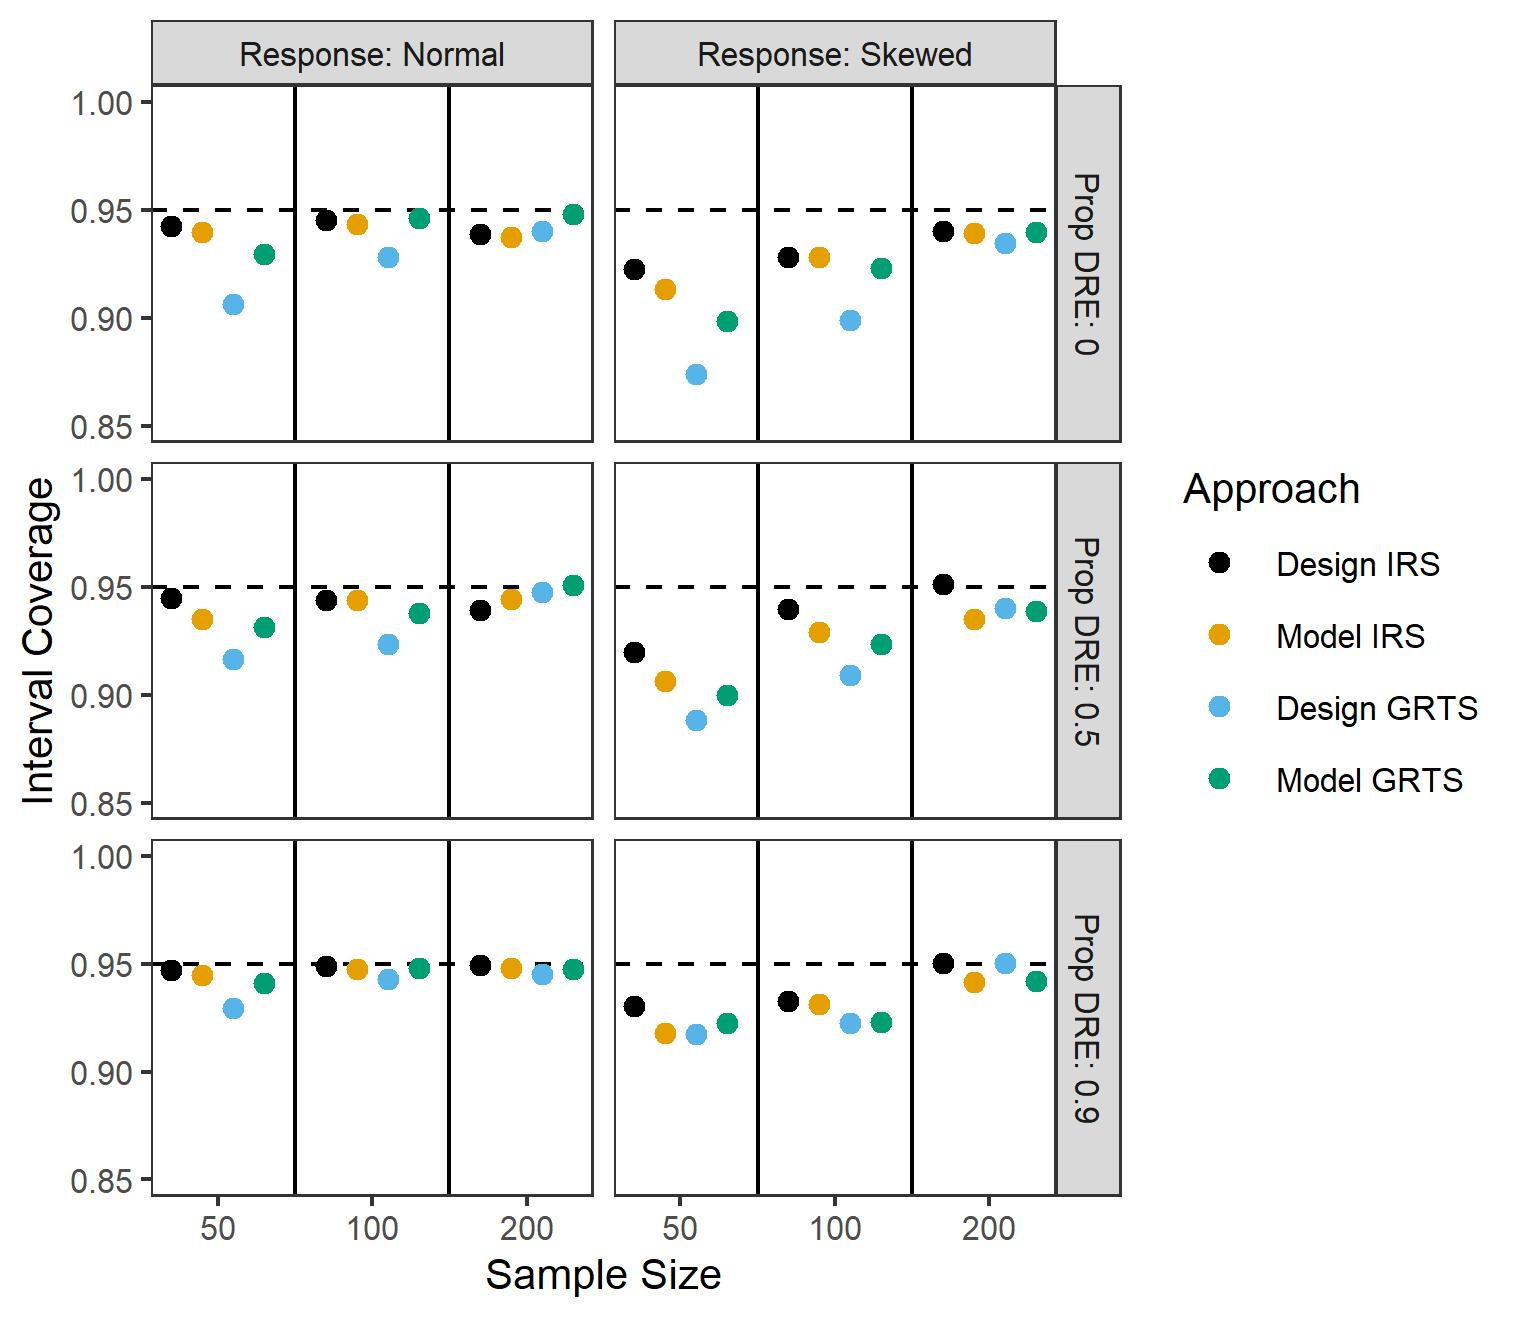
\includegraphics[width = 1\linewidth]{figures/coverage.jpeg}
  \caption{Interval coverage in the simulation study for the four sampling-inference combinations and three sample sizes in the random location layout. The rows indicate the proportion of dependent error and the columns indicate the response type. The solid black lines separate the sample sizes and the dashed black lines represent 95\% coverage.}
  \label{fig:figconf}
\end{figure}

\hypertarget{sec:r_app}{%
\subsection{National Lakes Assessment (Real) Data}\label{sec:r_app}}

Mean bias was nearly zero for all four sampling-inference combinations
in all six scenarios, so we omit a more detailed summary of those
results here. Tables for mean bias in all six simulations scenarios are
provided in the supporting information.

The relative RMSE of both ZMMI (symmetric response) and Hg ppb (skewed
response) for all four sampling-inference combinations are shown in
Fig.\(~\)\ref{fig:data_rmspe_eff}. GRTS-MB has the lowest RMSE, followed
by GRTS-DB, SRS-MB, and then SRS-DB. The difference in RMSE among
GRTS-MB and GRTS-DB tends to be quite small. When \(n = 50\), SRS-MB
RMSE is approximately evenly between IRS-DB RMSE and GRTS-MB RMSE, but
for the larger sample sizes (\(n = 100\), \(n = 200\)), SRS-MB RMSE is
closer to GRTS-MB RMSE. Lastly we note that GRTS-MB, GRTS-DB, and SRS-MB
all have noticeably lower RMSE than SRS-DB.

\begin{figure}
  \centering
  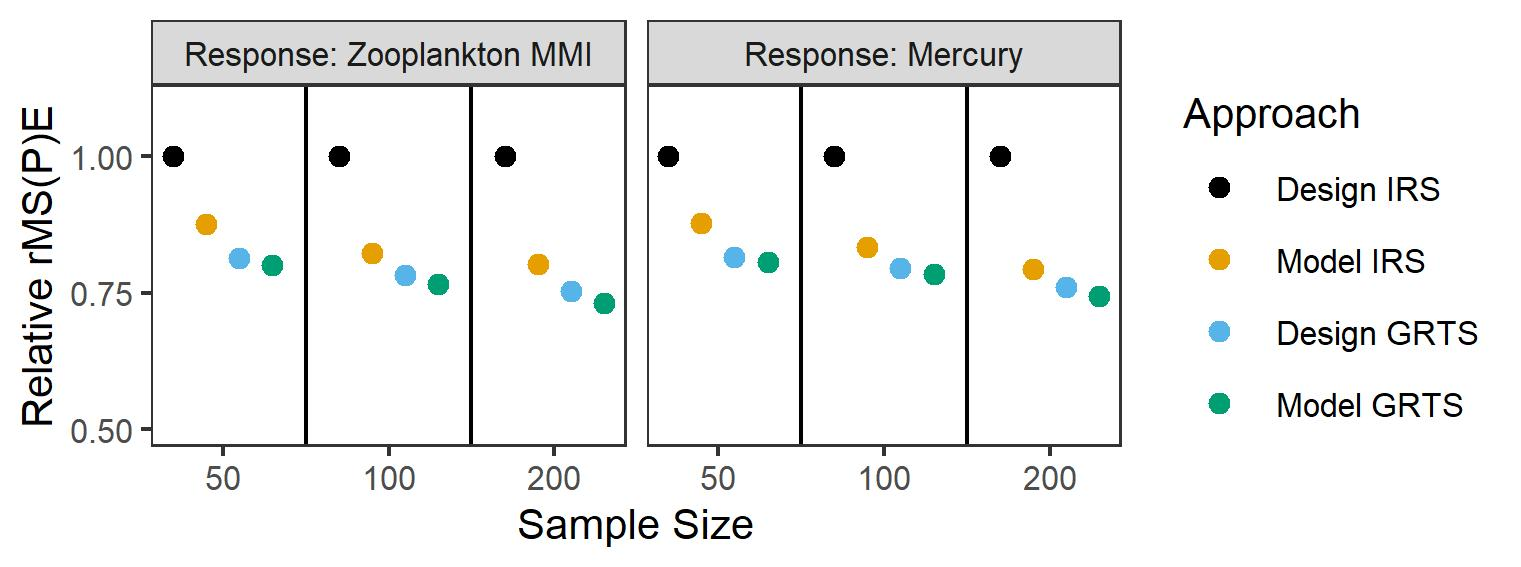
\includegraphics[width = 1\linewidth]{figures/data_rmspe_eff.jpeg}
  \caption{Relative RMSE in the data study for the four sampling-inference combinations. The rows indicate the proportion of dependent error and the columns indicate the response type. The solid, black lines separate the sample sizes.}
  \label{fig:data_rmspe_eff}
\end{figure}

95\% interval coverage of both ZMMI and Hg ppb for all four
sampling-inference combinations is shown in Fig. \ref{fig:figconf}. When
\(n = 50\), interval coverage for both responses is too low, though
interval coverage is higher for ZMMI (symmetric response) than for Hg
ppb (skewed response). When \(n = 100\), ZMMI interval coverage is
approximately 95\% except for GRTS-DB, which has coverage around 92\%,
while Hg ppb interval coverage ranges from approximately 90\% (GRTS-DB)
to 93\% (GRTS-MB). When \(n = 200\), ZMMI interval coverage is
approximately 95\% while Hg ppb interval coverage ranges from
approximately 93\% (GRTS-DB) to 95\% (GRTS-MB). As with the simulated
data, coverages for the NLA data tended to increase with the sample
sizes, coverages tended to be higher symmteric responses than skewed
responses, and regularly the local neighborhood variance was slightly
too small for small \(n\), yielding slightly lower interval coverages
than the other sampling-inference combinations. Recall that model-based
inference defines interval coverage properties across realized
populations. With the simulated data, we evaluated interval coverage
across realization populations, but for the NLA data, we evaluated
interval coverage within a single realization for different samples. We
did find that model-based coverages were similar to the design-based
coverages, however, suggesting that in many cases it is reasonable to
heuristically view data from separate samples as being from
approximately separate realized populations. But generally, if
model-based intervals constructed from many random samples of a single
realized population show improper coverage, this does not necessarily
imply a deficiency in model-based inference.

\begin{figure}
  \centering
  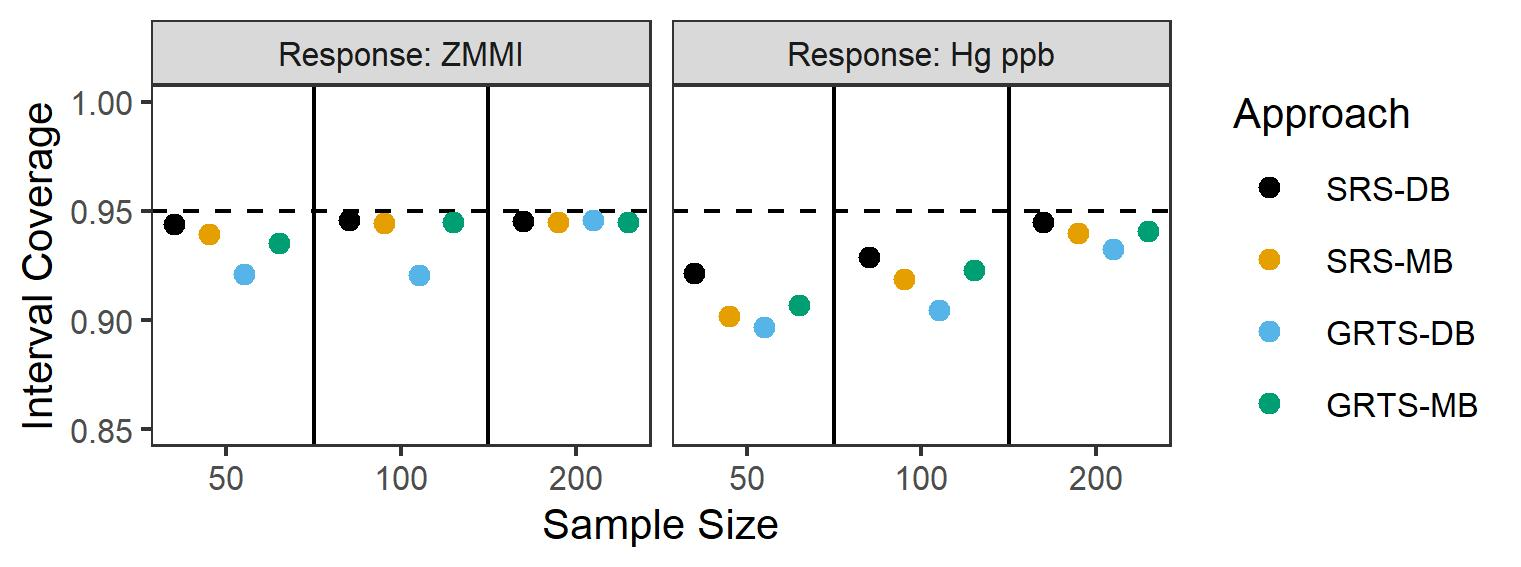
\includegraphics[width = 1\linewidth]{figures/data_coverage.jpeg}
  \caption{Interval coverage in the data study for the four sampling-inference combinations. The rows indicate the proportion of dependent error and the columns indicate the response type.The solid black lines separate the sample sizes and the dashed black lines represent 95\% coverage.}
  \label{fig:data_figconf}
\end{figure}

\hypertarget{sec:discussion}{%
\section{Discussion}\label{sec:discussion}}

ADD EXTRAS LIKE ANISOTROPY AND UNEQUAL INCLUSION PROBABILITIES

The design-based and model-based approaches to statistical inference are
fundamentally different paradigms. Design-based inference relies on
random sampling to estimate population parameters. Model-based inference
relies on distributional assumptions to predict realized values of a
data-generating stochastic process. Though model-based inference does
not rely on random sampling, it can still be beneficial as a way to
guard against preferential sampling. While design-based inference and
model-based inference have often been compared in the literature from
theoretical and analytical perspectives, our contribution lies in
studying them for finite population spatial data while implementing GRTS
sampling and the local neighborhood variance estimator. Aside from the
theoretical differences described throughout the manuscript, a few
analytical findings from the simulated and real data studies were
particularly notable. All sampling-inference combinations had
approximately zero mean bias. Independent of the inference approach,
GRTS-DB and GRTS-MB had lower RMSE than their SRS counterparts. Though
GRTS-DB and GRTS-MB generally had very similar RMSE, SRS-MB tended to
have much lower RMSE than SRS-DB, suggesting that the model-based
inference mitigated much of the inefficiency in RMSE from SRS. As the
proportion of dependent random error in the simulated data increased,
SRS-MB, GRTS-DB, and GRTS-MB become increasingly more efficient (lower
RMSE) than SRS-DB. Interval coverage tended to be higher for the
symmetric responses than skewed responses and tended to increase with
the sample size. At a sample size of \(n = 200\), generally all interval
coverages were near the desired value of 95\%.

There are several benefits and drawbacks of the design-based and
model-based approaches for finite population spatial data. Some we have
discussed, but others we have not, and they are worthy of consideration
in future research. First we discuss advantages of design-based
inference. Design-based inference is often computationally efficient,
while model-based inference can be computationally burdensome,
especially for likelihood-based estimation methods like REML that rely
on inverting a covariance matrix. Design-based inference easily handles
binary data through a straightforward application of the
Horvitz-Thompson estimator. In contrast, analyzing binary data using
model-based inference generally requires a logistic mixed regression
model, which can be difficult to estimate and interpret (Bolker et al.,
2009). An advantage of design-based inference is that interval coverage
is valid (has the proper coverage rate) as long as 1) the sample is
sufficiently large to ensure the statistic's sampling distribution is
approximately normal and 2) the variance estimator is consistent (Brus
and De Gruijter, 1997; Särndal et al., 2003). This is because with
design-based inference, the sampling plan and inclusion probabilities
are specified directly by the researcher. With the model-based approach,
however, interval coverage is unlikely to be valid if the model's
assumptions made do not not accurately reflect reality. Whether a
model's assumptions accurately reflect reality can be a challenging and
sometimes impossible question to answer definitively. Now we discuss
advantages of model-based inference. Model-based inference can more
naturally quantify the relationship between covariates (predictor
variables) and the response variable than design-based inference.
Model-based inference also yields estimated spatial covariance
parameters, which help better understand the dependence structure of the
process in study. Model selection is also possible using model-based
inference and criteria such as cross validation, likelihood ratio tests,
or AIC (Akaike, 1974). Model-based inference is capable of more
efficient small-area estimation than design-based inference because
model-based inference can leverage distributional assumptions in areas
with few observed population units. Model-based inference can also
compute unit-by-unit predictions at unobserved locations and use them to
construct informative visualizations like smoothed maps. Brus and De
Gruijter (1997) provide a more thorough discussion regarding the
benefits and drawbacks of the two approaches. In short, when deciding
whether the design-based or model-based approach is more appropriate to
implement, the benefits and drawbacks of each approach should be
considered alongside the particular goals of the study.

There are many extensions of this research worthy of future
consideration, some of which we discuss next. Some extensions to study
include sampling with unequal inclusion probabilities, different
spatially balanced sampling approaches (instead of GRTS), different
spatial data configurations, different spatial domains like stream
networks (Ver Hoef and Peterson, 2010), different response or covariance
structures, the effect of spatial or external mean trends (which can be
defined through covariates), and more.

\hypertarget{acknowledgments}{%
\section*{Acknowledgments}\label{acknowledgments}}
\addcontentsline{toc}{section}{Acknowledgments}

We would like to thank the editors and anonymous reviewers for their
thoughtful comments which greatly improved the manuscript.

The views expressed in this manuscript are those of the authors and do
not necessarily represent the views or policies of the U.S.
Environmental Protection Agency or the National Oceanic and Atmospheric
Administration. Any mention of trade names, products, or services does
not imply an endorsement by the U.S. government, the U.S. Environmental
Protection Agency, or the National Oceanic and Atmospheric
Administration. The U.S. Environmental Protection Agency and National
Oceanic and Atmospheric Administration do not endorse any commercial
products, services, or enterprises.

\hypertarget{conflict-of-interest-statement}{%
\section*{Conflict of Interest
Statement}\label{conflict-of-interest-statement}}
\addcontentsline{toc}{section}{Conflict of Interest Statement}

There are no conflicts of interest for any of the authors.

\hypertarget{author-contribution-statement}{%
\section*{Author Contribution
Statement}\label{author-contribution-statement}}
\addcontentsline{toc}{section}{Author Contribution Statement}

All authors conceived the ideas; All authors designed the methodology;
MD and MH performed the simulations and analyzed the data; MD and MH led
the writing of the manuscript; All authors contributed critically to the
drafts and gave final approval for publication.

\hypertarget{data-and-code-availability}{%
\section*{Data and Code Availability}\label{data-and-code-availability}}
\addcontentsline{toc}{section}{Data and Code Availability}

This manuscript has a supplementary \textbf{\textsf{R}} package that
contains all of the data and code used in its creation. The
supplementary \textbf{\textsf{R}} package is hosted on GitHub.
Instructions for download at available at

\url{https://github.com/michaeldumelle/DvMsp}.

If the manuscript is accepted, this repository will be archived in
Zenodo.

\hypertarget{supporting-information}{%
\section*{Supporting Information}\label{supporting-information}}
\addcontentsline{toc}{section}{Supporting Information}

In the supporting information, we provide tables of summary statistics
for all 36 simulation scenarios.

\hypertarget{references}{%
\section*{References}\label{references}}
\addcontentsline{toc}{section}{References}

\hypertarget{refs}{}
\leavevmode\hypertarget{ref-akaike1974new}{}%
Akaike, H., 1974. A new look at the statistical model identification.
IEEE Transactions on Automatic Control 19, 716--723.

\leavevmode\hypertarget{ref-barabesi2011sampling}{}%
Barabesi, L., Franceschi, S., 2011. Sampling properties of spatial total
estimators under tessellation stratified designs. Environmetrics 22,
271--278.

\leavevmode\hypertarget{ref-benedetti2017spatially}{}%
Benedetti, R., Piersimoni, F., 2017. A spatially balanced design with
probability function proportional to the within sample distance.
Biometrical Journal 59, 1067--1084.

\leavevmode\hypertarget{ref-benedetti2017spatiallyreview}{}%
Benedetti, R., Piersimoni, F., Postiglione, P., 2017. Spatially balanced
sampling: A review and a reappraisal. International Statistical Review
85, 439--454.

\leavevmode\hypertarget{ref-bolker2009generalized}{}%
Bolker, B.M., Brooks, M.E., Clark, C.J., Geange, S.W., Poulsen, J.R.,
Stevens, M.H.H., White, J.-S.S., 2009. Generalized linear mixed models:
A practical guide for ecology and evolution. Trends in ecology \&
evolution 24, 127--135.

\leavevmode\hypertarget{ref-breiman2001random}{}%
Breiman, L., 2001. Random forests. Machine Learning 45, 5--32.

\leavevmode\hypertarget{ref-brus1997random}{}%
Brus, D., De Gruijter, J., 1997. Random sampling or geostatistical
modelling? Choosing between design-based and model-dased sampling
strategies for soil (with discussion). Geoderma 80, 1--44.

\leavevmode\hypertarget{ref-brus2021statistical}{}%
Brus, D.J., 2021. Statistical approaches for spatial sample survey:
Persistent misconceptions and new developments. European Journal of Soil
Science 72, 686--703.

\leavevmode\hypertarget{ref-brus1993design}{}%
Brus, D.J., DeGruijter, J.J., 1993. Design-based versus model-based
estimates of spatial means: Theory and application in environmental soil
science. Environmetrics 4, 123--152.

\leavevmode\hypertarget{ref-chan2020bayesian}{}%
Chan-Golston, A.M., Banerjee, S., Handcock, M.S., 2020. Bayesian
inference for finite populations under spatial process settings.
Environmetrics 31, e2606.

\leavevmode\hypertarget{ref-chiles1999geostatistics}{}%
Chiles, J.-P., Delfiner, P., 1999. Geostatistics: Modeling Spatial
Uncertainty. John Wiley \& Sons, New York.

\leavevmode\hypertarget{ref-cicchitelli2012model}{}%
Cicchitelli, G., Montanari, G.E., 2012. Model-assisted estimation of a
spatial population mean. International Statistical Review 80, 111--126.

\leavevmode\hypertarget{ref-cooper2006sampling}{}%
Cooper, C., 2006. Sampling and variance estimation on continuous
domains. Environmetrics 17, 539--553.

\leavevmode\hypertarget{ref-cressie1993statistics}{}%
Cressie, N., 1993. Statistics for spatial data. John Wiley \& Sons.

\leavevmode\hypertarget{ref-de1990model}{}%
De Gruijter, J., Ter Braak, C., 1990. Model-free estimation from spatial
samples: A reappraisal of classical sampling theory. Mathematical
Geology 22, 407--415.

\leavevmode\hypertarget{ref-diggle2010geostatistical}{}%
Diggle, P.J., Menezes, R., Su, T.-l., 2010. Geostatistical inference
under preferential sampling. Journal of the Royal Statistical Society:
Series C (Applied Statistics) 59, 191--232.

\leavevmode\hypertarget{ref-dumelle2022spsurvey}{}%
Dumelle, M., Kincaid, T.M., Olsen, A.R., Weber, M.H., 2022. Spsurvey:
Spatial sampling design and analysis.

\leavevmode\hypertarget{ref-fix1989discriminatory}{}%
Fix, E., Hodges, J.L., 1989. Discriminatory analysis. Nonparametric
discrimination: Consistency properties. International Statistical
Review/Revue Internationale de Statistique 57, 238--247.

\leavevmode\hypertarget{ref-grafstrom2012spatiallypoisson}{}%
Grafström, A., 2012. Spatially correlated poisson sampling. Journal of
Statistical Planning and Inference 142, 139--147.

\leavevmode\hypertarget{ref-grafstrom2013well}{}%
Grafström, A., Lundström, N.L., 2013. Why well spread probability
samples are balanced. Open Journal of Statistics 3, 36--41.

\leavevmode\hypertarget{ref-grafstrom2012spatially}{}%
Grafström, A., Lundström, N.L., Schelin, L., 2012. Spatially balanced
sampling through the pivotal method. Biometrics 68, 514--520.

\leavevmode\hypertarget{ref-grafstrom2018spatially}{}%
Grafström, A., Matei, A., 2018. Spatially balanced sampling of
continuous populations. Scandinavian Journal of Statistics 45, 792--805.

\leavevmode\hypertarget{ref-hansen1983evaluation}{}%
Hansen, M.H., Madow, W.G., Tepping, B.J., 1983. An evaluation of
model-dependent and probability-sampling inferences in sample surveys.
Journal of the American Statistical Association 78, 776--793.

\leavevmode\hypertarget{ref-harville1977maximum}{}%
Harville, D.A., 1977. Maximum likelihood approaches to variance
component estimation and to related problems. Journal of the American
Statistical Association 72, 320--338.

\leavevmode\hypertarget{ref-hofman2021many}{}%
Hofman, S.C., Brus, D., 2021. How many sampling points are needed to
estimate the mean nitrate-n content of agricultural fields? A
geostatistical simulation approach with uncertain variograms. Geoderma
385, 114816.

\leavevmode\hypertarget{ref-horvitz1952generalization}{}%
Horvitz, D.G., Thompson, D.J., 1952. A generalization of sampling
without replacement from a finite universe. Journal of the American
Statistical Association 47, 663--685.

\leavevmode\hypertarget{ref-lohr2009sampling}{}%
Lohr, S.L., 2009. Sampling: Design and analysis. Nelson Education.

\leavevmode\hypertarget{ref-patterson1971recovery}{}%
Patterson, H.D., Thompson, R., 1971. Recovery of inter-block information
when block sizes are unequal. Biometrika 58, 545--554.

\leavevmode\hypertarget{ref-robertson2013bas}{}%
Robertson, B., Brown, J., McDonald, T., Jaksons, P., 2013. BAS: Balanced
acceptance sampling of natural resources. Biometrics 69, 776--784.

\leavevmode\hypertarget{ref-robertson2018halton}{}%
Robertson, B., McDonald, T., Price, C., Brown, J., 2018. Halton
iterative partitioning: Spatially balanced sampling via partitioning.
Environmental and Ecological Statistics 25, 305--323.

\leavevmode\hypertarget{ref-sarndal2003model}{}%
Särndal, C.-E., Swensson, B., Wretman, J., 2003. Model assisted survey
sampling. Springer Science \& Business Media.

\leavevmode\hypertarget{ref-schabenberger2017statistical}{}%
Schabenberger, O., Gotway, C.A., 2017. Statistical methods for spatial
data analysis. CRC press.

\leavevmode\hypertarget{ref-sen1953estimate}{}%
Sen, A.R., 1953. On the estimate of the variance in sampling with
varying probabilities. Journal of the Indian Society of Agricultural
Statistics 5, 127.

\leavevmode\hypertarget{ref-sterba2009alternative}{}%
Sterba, S.K., 2009. Alternative model-based and design-based frameworks
for inference from samples to populations: From polarization to
integration. Multivariate Behavioral Research 44, 711--740.

\leavevmode\hypertarget{ref-stevens2003variance}{}%
Stevens, D.L., Olsen, A.R., 2003. Variance estimation for spatially
balanced samples of environmental resources. Environmetrics 14,
593--610.

\leavevmode\hypertarget{ref-stevens2004spatially}{}%
Stevens, D.L., Olsen, A.R., 2004. Spatially balanced sampling of natural
resources. Journal of the American Statistical Association 99, 262--278.

\leavevmode\hypertarget{ref-USEPA2012NLA}{}%
USEPA, 2012. National lakes assessment 2012.
https://www.epa.gov/national-aquatic-resource-surveys/national-results-and-regional-highlights-national-lakes-assessment.

\leavevmode\hypertarget{ref-verhoef2002sampling}{}%
Ver Hoef, J., 2002. Sampling and geostatistics for spatial data.
Ecoscience 9, 152--161.

\leavevmode\hypertarget{ref-verhoef2008spatial}{}%
Ver Hoef, J.M., 2008. Spatial methods for plot-based sampling of
wildlife populations. Environmental and Ecological Statistics 15, 3--13.

\leavevmode\hypertarget{ref-ver2010moving}{}%
Ver Hoef, J.M., Peterson, E.E., 2010. A moving average approach for
spatial statistical models of stream networks. Journal of the American
Statistical Association 105, 6--18.

\leavevmode\hypertarget{ref-ver2013comparison}{}%
Ver Hoef, J.M., Temesgen, H., 2013. A comparison of the spatial linear
model to nearest neighbor (k-nn) methods for forestry applications. PlOS
ONE 8, e59129.

\leavevmode\hypertarget{ref-walvoort2010r}{}%
Walvoort, D.J., Brus, D., De Gruijter, J., 2010. An r package for
spatial coverage sampling and random sampling from compact geographical
strata by k-means. Computers \& geosciences 36, 1261--1267.

\leavevmode\hypertarget{ref-wang2013design}{}%
Wang, J.-F., Jiang, C.-S., Hu, M.-G., Cao, Z.-D., Guo, Y.-S., Li, L.-F.,
Liu, T.-J., Meng, B., 2013. Design-based spatial sampling: Theory and
implementation. Environmental Modelling \& Software 40, 280--288.

\leavevmode\hypertarget{ref-wolfinger1994computing}{}%
Wolfinger, R., Tobias, R., Sall, J., 1994. Computing gaussian
likelihoods and their derivatives for general linear mixed models. SIAM
Journal on Scientific Computing 15, 1294--1310.


\end{document}

